%& --translate-file=cp1250pl.tcx
\documentclass[10pt,a4paper]{book}
\usepackage{polski}
\usepackage{amsmath}
\usepackage{amsfonts}
\usepackage{amssymb}
\usepackage{graphicx}
\usepackage{verbatim}
\usepackage{hyperref}
\usepackage{todonotes}
\author{Jakub Mozaryn, Jan Klimaszewski}
\title{Sterowanie Mechanizm�w Wielocz�onowych}
\begin{document}
	\maketitle
	\tableofcontents
	
	%ROZDZIA�Y
	
%ROZDZIA� 1
\chapter{Opis mechanizm�w wielocz�onowych - Janek+Kuba}
  W rozdziale przedstawiono podstawy matematyczne i fizyczne s�u��ce do opisu
  robot�w o wielu stopniach swobody (mechniazm�w wielocz�onowych). Przedstawiono model robota w przestrzeni zmiennych stanu. Opisano spos�b symulacji komputerowej dynamiki robota.	
  
  \subsubsection{Mechanizm wielocz�onowy}
  Mechanizm jest to zesp� wsp�pracuj�cych ze sob� cz�ci sk�adowych maszyny lub przyrz�du spe�niaj�cych okre�lone zadanie, jak np. przenoszenie ruchu, si�, sygna��w[1].
  Mechanizm wielocz�onowy jest to zesp� po��czonych sztywnych lub elastycznych bry�. Po��czenia pozwalaj� na zmian� wzajemnego po�o�enia pomi�dzy po��czonymi bry�ami.\footnote{\url{https://en.wikipedia.org/wiki/Multibody_system}}\\
  \todo{Doda� przyk�ad z obrazkiem - 2-link planar robotic arm - rysunek, ewentualnie przenie�� to jeszcze wcze�niej - Mo�e da� to jako element rozdzia�u "Wprowadzenie"?}
  
  
  \section{Wprowadzenie matematyczne - Janek}
  \todo{Przenie�� to do za��cznika?}
  
  \subsubsection{Podstawowe poj�cia}
  
  Geometry is a branch of mathematics concerned with questions of shape, size, relative position of figures, and the properties of space. \footnote{https://en.wikipedia.org/wiki/Geometry}
  
  Kinematics is a branch of classical mechanics that describes the motion of points, bodies (objects), and systems of bodies (groups of objects) without considering the mass of each or the forces that caused the motion.[1][2][3] Kinematics, as a field of study, is often referred to as the "geometry of motion" and is occasionally seen as a branch of mathematics.[4][5][6] A kinematics problem begins by describing the geometry of the system and declaring the initial conditions of any known values of position, velocity and/or acceleration of points within the system. Then, using arguments from geometry, the position, velocity and acceleration of any unknown parts of the system can be determined. \footnote{\url{https://en.wikipedia.org/wiki/Kinematics}}
  
  Dynamika = Kinetyka. In classical mechanics, analytical dynamics, or more briefly dynamics, is concerned with the relationship between motion of bodies and its causes, namely the forces acting on the bodies and the properties of the bodies, particularly mass and moment of inertia. The foundation of modern-day dynamics is Newtonian mechanics and its reformulation as Lagrangian mechanics and Hamiltonian mechanics.[1][2] \footnote{\url{https://en.wikipedia.org/wiki/Kinetics_(physics)}}\footnote{\url{https://en.wikipedia.org/wiki/Analytical_dynamics}}\\
  
    
  \subsubsection{Operacje macierzowe}
  odwracanie\\
  ortogonalno��\\
  niezale�no�� r�wna�\\
  r�niczkowanie\\
  pochodne cz�stkowe\\
  
  \subsubsection{Podstawy geometrii analitycznej}
    Analytic geometry is the study of geometry on a grid called the coordinate plane, or xyz-plane. \\
    Uk�ad wsp�rz�dnych. W szczeg�lno�ci kartezja�ski.\\
    Punkt. Wektor.\\
    Powierzchnia. P�aszczyzna. R�wnanie precyzuje zwykle powierzchni�.\\
    Linia.\\
    Odleg�o�� i k�t.\\
    Rzuty\\
    , prostopad�o��, r�wnoleg�o��, przeci�cia itp.\\
    Bry�a sztywna = rigid body\\
    Degree of freedom\\
    The degrees of freedom denote the number of independent kinematical possibilities to move. In other words, degrees of freedom are the minimum number of parameters required to completely define the position of an entity in space.\\
    A rigid body has six degrees of freedom in the case of general spatial motion, three of them translational degrees of freedom and three rotational degrees of freedom. In the case of planar motion, a body has only three degrees of freedom with only one rotational and two translational degrees of freedom.\\
    
  \subsubsection{Podstawowe transformacje uk�ad�w wsp�rz�dnych}
  Elementarne macierze transformacji � macierze opisuj�ce zale�no�� pomi�dzy wsp�rz�dnymi wskazanego punktu przed i po transformacji. Przez transformacj� rozumiemy w tym przypadku translacj� (czyli przesuni�cie), skalowanie oraz rotacj� (czyli obr�t). W przypadku opisu mechanizm�w wielocz�onych sens fizyczny maj� zazwyczaj tylko operacje translacji o rotacji - tylko one b�d� omawiane.

  Transformacje maj� najcz�ciej o jeden rz�d wi�cej ni� wymiar wektora wsp�rz�dnych, a dok�adniej maj� rz�d r�wny wymiarowi wsp�rz�dnych jednorodnych\todo{wyjasnic gdzies co to jest}. \footnote{\url{https://pl.wikipedia.org/wiki/Elementarne_macierze_transformacji}}
    
\textbf{Elementarne macierze translacji}\\
W tym przypadku trzy przesuni�cia mog� zosta� zapisane jako jedna macierz, poniewa� r�ni� si� tylko ostatni� kolumn�.

\begin{equation}
Tran( a, b, c ) = \begin{bmatrix} 1 & 0 & 0 & a \\ 0 & 1 & 0 & b \\ 0 & 0 & 1 & c \\ 0 & 0 & 0 & 1 \end{bmatrix}
\end{equation}
gdzie: 
$a, b, c$ - przesuni�cie wzd�u� osi $X, Y$ oraz $Z$

Mo�na tak�e rozbi� t� macierz na 3 osobne: $TranX(a)$, $TranY(b)$ oraz $TranZ(c)$.
    
\textbf{Elementarne macierze rotacji}\\
Obroty przedstawiane s� w r�ny spos�b, dlatego te� elementarne macierze rotacji musz� by� przedstawiane oddzielnie.

Dla osi X:
\begin{equation}
RotX(\alpha)=
\begin{bmatrix}
  1 & 0 & 0 & 0 \\
  0 & \cos\alpha & -\sin\alpha & 0 \\
  0 & \sin\alpha & \cos\alpha & 0 \\
  0 & 0 & 0 & 1 \\
\end{bmatrix}
\end{equation}

Dla osi Y:
\begin{equation}
RotY(\beta)=
\begin{bmatrix}
  \cos\beta & 0 & \sin\beta & 0 \\
  0 & 1 & 0 & 0 \\
  -\sin\beta & 0 & \cos\beta & 0 \\
  0 & 0 & 0 & 1 \\
\end{bmatrix}
\end{equation}

Dla osi Z:
\begin{equation}
RotZ(\gamma)=
\begin{bmatrix}
  \cos\gamma & -\sin\gamma & 0 & 0 \\
  \sin\gamma & \cos\gamma & 0 & 0 \\
  0 & 0 & 1 & 0 \\
  0 & 0 & 0 & 1 \\
\end{bmatrix}
\end{equation}

\textbf{Sk�adanie macierzy}\\
Istnieje mo�liwo�� sk�adania transformacji. W�wczas obliczamy macierz wynikow� b�d�c� iloczynem sk�adowych macierzy transformacji, kt�r� "dzia�amy" na dany punkt w przestrzeni.

\begin{equation}
\begin{bmatrix} x' \\ y' \\ z' \\ 1 \end{bmatrix} = 
\begin{bmatrix} 1 & 0 & 0 & a \\ 0 & 1 & 0 & b \\ 0 & 0 & 1 & c \\ 0 & 0 & 0 & 1 \end{bmatrix}
\begin{bmatrix}
  \cos\gamma & -\sin\gamma & 0 & 0 \\
  \sin\gamma & \cos\gamma & 0 & 0 \\
  0 & 0 & 1 & 0 \\
  0 & 0 & 0 & 1 \\
\end{bmatrix}
\begin{bmatrix} x \\ y \\ z \\ 1 \end{bmatrix}
\end{equation}

W powy�szym przyk�adzie najpierw wykonujemy operacj� rotacji, nast�pnie translacji o wektor. Takich operacji mo�e by� wi�cej. Ka�d� nast�pn� macierz transformacji dok�adamy po lewej stronie iloczynu macierzy, przy czym mno�enie macierzy przez wektor wykonujemy od prawej strony do lewej.

Mo�emy tak�e powy�sz� operacj� zast�pi� iloczynem macierzy wynikowej przez wektor. 

\begin{equation}
\begin{bmatrix} x' \\ y' \\ z' \\ 1 \end{bmatrix} = 
M
\begin{bmatrix} x \\ y \\ z \\ 1 \end{bmatrix}
\end{equation},

Macierz transformacji b�d�c� z�o�eniem poszczeg�lnych transformacji sk�adowych otrzymamy ze wzoru.

\begin{equation}
M = 
\begin{bmatrix} 1 & 0 & 0 & a \\ 0 & 1 & 0 & b \\ 0 & 0 & 1 & c \\ 0 & 0 & 0 & 1 \end{bmatrix}
\begin{bmatrix}
  \cos\gamma & -\sin\gamma & 0 & 0 \\
  \sin\gamma & \cos\gamma & 0 & 0 \\
  0 & 0 & 1 & 0 \\
  0 & 0 & 0 & 1 \\
\end{bmatrix}
\end{equation},

Gdy s� dane dwie (lub wi�cej) macierze przekszta�ce�:
\begin{itemize}
\item $Rot^0_1$ - macierz przekszta�caj�ca zerowy uk�ad wsp�rz�dnych w uk�ad o indeksie pierwszym.
\item $Rot^1_2$ - macierz przekszta�caj�ca uk�ad pierwszy w uk�ad drugi.
\end{itemize}
Obydwie macierze mo�na z�o�y� w jedn� macierz przekszta�caj�c� uk�ad zerowy w uk�ad drugi.
$Rot^0_2=Rot^0_1*Rot^1_2$

Macierze te oraz ich [[mno�enie macierzy|iloczyn]] nale�y do specjalnej grupy euklidesowej SE(3). 

\textbf{Specjalna grupa euklidesowa}\\
Specjalna grupa euklidesowa SE(3) to zbi�r [[macierz]]y $\begin{bmatrix} R & T \\ 0 & 1 \end{bmatrix}$ (gdzie R to macierz opisuj�ca obr�t, a T to macierz opisuj�ca [[translacja (matematyka)|translacj�]]), kt�re spe�niaj� warunki:
\begin{itemize}
\item \begin{equation}\begin{bmatrix} R & T \\ 0 & 1 \end{bmatrix}^{-1} \begin{bmatrix} R & T \\ 0 & 1 \end{bmatrix} = I_4\end{equation}
\item \begin{equation}\begin{bmatrix} R & T \\ 0 & 1 \end{bmatrix}^{-1} = \begin{bmatrix} R^T & -R^TT \\ 0 & 1 \end{bmatrix}\end{equation}
\item \begin{equation}\begin{bmatrix} R_1 & T_1 \\ 0 & 1 \end{bmatrix}\begin{bmatrix} R_2 & T_2 \\ 0 & 1 \end{bmatrix} = \begin{bmatrix} R_1R_2 & R_1T_2+T_1 \\ 0 & 1 \end{bmatrix} \in SE(3)\end{equation}
\end{itemize}

Specjalna grupa euklidesowa mo�e by� tak�e zapisana jako iloczyn [[wektor]]a oraz [[grupa obrot�w|grupy obrot�w]] tj. $SE(3) \cong R^3 \times SO(3)$.

Macierze nale��ce do SE(3) pozwalaj� opisa� [[Ruch (fizyka)|ruch]] [[bry�a sztywna|cia�a sztywnego]]. Do ich konstrukcji wykorzystane mog� by� elementarne macierze transformacji. Przy takim zapisie macierzy konieczne jest tak�e stosowanie [[wsp�rz�dne jednorodne|wsp�rz�dnych jednorodnych]], �eby wymiar [[wektor]]a wsp�rz�dnych by� r�wny liczbie kolumn macierzy. 

\textbf{Interpretacje}\\
Macierze nale��ce do SE(3) pozwalaj�:
\begin{itemize}
\item przekszta�ci� punkt P w Q wzgl�dem ustalonego [[uk�ad wsp�rz�dnych|uk�adu]] $(X_0,Y_0,Z_0)$
\item przekszta�ci� uk�ad $(X_0,Y_0,Z_0)$ w taki uk�ad $(X_1,Y_1,Z_1)$, �e wsp�rz�dne punktu $\begin{bmatrix} x & 1 \end{bmatrix}^T$ wzgl�dem $(X_1,Y_1,Z_1)$ transformuj� si� do uk�adu $(X_0,Y_0,Z_0)$ jako:
\begin{equation}\begin{bmatrix} R & T \\ 0 & 1 \end{bmatrix} \begin{bmatrix} x \\ 1 \end{bmatrix}\end{equation}
\end{itemize}
  
  
  \section{Model geometrii, kinematyki i dynamiki mechanizm�w wielocz�onowych.}

  \subsection{Model geometrii - Janek}
  W pracy rozwa�any jest robot o pojedynczym �a�cuchu kinematycznym, sk�adaj�cy
  si� z cz�on�w po��czonych przegubami. Ka�dy z przegub�w posiada jeden stopie� swobody. W dalszej cz�ci pracy rozwa�any b�dzie robot o $n$-stopniach swobody z przegubami typu obrotowego, gdy� tylko przeguby tego typu wyst�puj� w rozwa�anym w pracy robocie PUMA 560. Przyj�to, �e dla robota o $n$-przegubach ponumerowanych od 1 do $n$ istnieje $n$+1 cz�on�w ponumerowanych od 0 do $n$. Cz�on o numerze 0 nazywany jest cz�onem bazowym, natomiast cz�on $n$ jest cz�onem z elementem wykonawczym. Przegub i ��czy cz�ony o numerach $i$-1 i $i$. Z ka�dym z cz�on�w zwi�zany jest uk�ad wsp�rz�dnych o tym samym numerze.
  Rozwa�amy mechanizm wielocz�onowy sk�adaj�cy si� z cz�on�w po��czonych stawami. Mog� wyst�powa� cz�ony nieruchome.\\
  
  \subsubsection{Cz�on}
  A body is usually considered to be a rigid or flexible part of a mechanical system. An example of a body is the arm of a robot, a wheel or axle in a car or the human forearm.\\
  
  \subsubsection{Staw, przegub}
  A link is the connection of two or more bodies, or a body with the ground. The link is defined by certain (kinematical) constraints that restrict the relative motion of the bodies. Typical constraints are:\\
    cardan joint or Universal Joint ; 4 kinematical constraints\\
    prismatic joint; relative displacement along one axis is allowed, constrains relative rotation; implies 5 kinematical constraints\\
    revolute joint; only one relative rotation is allowed; implies 5 kinematical constraints; see the example above\\
    spherical joint; constrains relative displacements in one point, relative rotation is allowed; implies 3 kinematical constraints\\
  Constraint condition\\
 A constraint condition implies a restriction in the kinematical degrees of freedom of one or more bodies. The classical constraint is usually an algebraic equation that defines the relative translation or rotation between two bodies. There are furthermore possibilities to constrain the relative velocity between two bodies or a body and the ground. This is for example the case of a rolling disc, where the point of the disc that contacts the ground has always zero relative velocity with respect to the ground. In the case that the velocity constraint condition cannot be integrated in time in order to form a position constraint, it is called non-holonomic. This is the case for the general rolling constraint.  

  \subsubsection{Mechanizm wielocz�onowy}
  �a�cuch kinematyczny jest to cz�� mechanizmu w postaci kilku po��czonych ze sob� cz�on�w (bry�) tworz�cych jedn� lub wiele par kinematycznych, realizuj�cy zdefiniowane przeniesienie ruchu.
  Model geometrii - zestaw cz�on�w i staw�w. �a�cuch kinematyczny.\\
    Stopnie swobody i wi�zy w uj�ciu mechanizmu wielocz�onowego, wi�zy bierne, nadmiarowe?\\
    Ruchliwo��\\
    Notacja DH.\\
    Zadanie proste geometrii.\\
    Zadanie odwrotne geometrii.\\
    
      Dla okre�lenia uk�ad�w wsp�rz�dnych kartezja�skich, kt�re b�d� przyporz�dkowane
  w odpowiedni spos�b do cz�on�w i przegub�w przyj�to notacj� Denavita-Hartenberga
  \cite{hartenberg:1955}, kt�rej podstawy zamieszczono na Rys. \ref{fig:1}:

  \begin{figure}[htb!]
	  \begin{center}
		  \includegraphics[width=1\linewidth]{figures/fig1}
		  %\\[1em]%
		  \caption{Standardowa notacja Denavita � Hartenberga (przyk�ad dw�ch obrotowych przegub�w $i$-1 oraz $i$), $a_i$ - d�ugo�� cz�onu, odleg�o�� od osi $z_i-1$ do osi $z_i$ mierzona wzd�u� osi $x_i$, $\alpha_i$ � k�t skr�cenia, k�t mi�dzy osiami $z_i-1$ i $z_i$ mierzony wok� osi $x_i$, $d_i$ - odsuni�cie cz�on�w,
			  odleg�o�� od �rodka uk�adu $i-1$ do osi $x_i$ mierzona wzd�u� osi $z_i-1$, $\theta_i$ - k�t konfiguracji, k�t mi�dzy osiami $x_i-1$ i $x_i$ mierzony wok� osi $z_i-1$ } \label{fig:1}
	  \end{center}                                         
  \end{figure}

  Po okre�leniu parametr�w uk�ad�w wsp�rz�dnych kartezja�skich mo�na wyznaczy�
  jednorodne macierze przekszta�ce� okre�laj�cych orientacj� i po�o�enie uk�adu $i$ wzgl�dem uk�adu $i-1$ \cite{fu:1987}:

  \begin{equation}
  ^{i-1}T{i}=T_{z,\theta}T_{z,d}T_{x,a}T_{x,\alpha}
  \end{equation}\label{eq:1}
  %
  gdzie: $^{i-1}T{i}$ - jednorodna macierz przekszta�cenia uk�adu $i-1$ wzgl�dem uk�adu $i$,$T_{z,\theta}$ - jednorodna macierz obrotu uk�adu $i$ wzgl�dem uk�adu $i-1$ wok� osi $z_i-1$ o k�t $\theta_i$, $T_{z,d}$ - jednorodna macierz przesuni�cia uk�adu $i$ wzgl�dem uk�adu $i-1$ o $d_i$ wzd�u� osi $z_i-1$,$T_{x,a}$ -  jednorodna macierz przesuni�cia uk�adu $i$ wzgl�dem uk�adu $i-1$ o $a_i$ wzd�u� osi $x_i$. ,$T_{x,\alpha}$-jednorodna macierz obrotu uk�adu $i$ wzgl�dem uk�adu $i-1$ wok� osi $x_i$ o k�t $\alpha_i$. 

  Macierze te wyra�one s� nast�puj�cymi zale�no�ciami:
  %
  \begin{equation}
  T_{z,\theta}=\left[\begin{array}{cccc}
  \cos{\theta_i} & -\sin{\theta_i} & 0 & 0 \\ 
  \sin{\theta_i} & \cos{\theta_i} & 0 & 0 \\ 
  0 & 0 & 1 & 0 \\ 
  0 & 0 & 0 & 1
  \end{array}\right] 
  \end{equation}\label{eq:2}
  %
  \begin{equation}
  T_{z,d}=\left[\begin{array}{cccc}
  1 & 0 & 0 & 0 \\ 
  0 & 1 & 0 & 0 \\ 
  0 & 0 & 1 & d_{i} \\ 
  0 & 0 & 0 & 1
  \end{array}\right] 
  \end{equation}\label{eq:3}
  %
  \begin{equation}
  T_{x,a}=\left[\begin{array}{cccc}
  1 & 0 & 0 & a_{i} \\ 
  0 & 1 & 0 & 0 \\ 
  0 & 0 & 1 & 0 \\ 
  0 & 0 & 0 & 1
  \end{array}\right] 
  \end{equation}\label{eq:4}
  %
  \begin{equation}
  T_{x,\alpha}=\left[\begin{array}{cccc}
  1 & 0 & 0 & 0 \\ 
  0 & \cos{\alpha_i} & -\sin{\alpha_i} & 0 \\ 
  0 & \sin{\alpha_i} & \cos{\alpha_i} & 0 \\ 
  0 & 0 & 0 & 1
  \end{array}\right] 
  \end{equation}\label{eq:5}
  %
  Wykorzystuj�c jednorodne macierze przekszta�ce� mo�na obliczy� wsp�rz�dne
  punktu w $m$-tym uk�adzie, znaj�c wsp�rz�dne tego samego punktu w $k$-tym uk�adzie
  (zak�adaj�c, �e $k>m$), jest to tzw. proste zadanie kinematyki. Zale�no�� t� wyznacza si�
  korzystaj�c z wyra�enia \cite{fu:1987}:
  %
  \begin{equation}
  P_{Am}=^{m}T_{k}P_{Ak}, k>m
  \end{equation}\label{eq:6}
  %
  gdzie:
  %
  \begin{equation}
  ^{m}T_{k}=^{m}T_{m+1}\quad ^{m+1}T_{m+2} \dots ^{k-1}T_{k}
  \end{equation}\label{eq:7}
  %
  $P_{Ak}=\left[\begin{array}{c}
  x_{Ak}\\ 
  y_{Ak}\\ 
  z_{Ak}\\ 
  1
  \end{array}\right]$ - jednorodny wektor wsp�rz�dnych punktu $A$ w $k$-tym uk�adzie wsp�rz�dnych

  $P_{Am}=\left[\begin{array}{c}
  x_{Am}\\ 
  y_{Am}\\ 
  z_{Am}\\ 
  1
  \end{array}\right]$ - jednorodny wektor wsp�rz�dnych punktu $A$ w $m$-tym uk�adzie wsp�rz�dnych
  %
    
  %
  \subsection{Model kinematyki - Janek}

  
  \subsection{Model dynamiki - Kuba}
  %
  Zale�no�ci opisuj�ce dynamik� robota o $n$-stopniach swobody mo�na wyznaczy�
  wykorzystuj�c uog�lnione r�wnanie Lagrange�a - Eulera o postaci \cite{fu:1987}
  %
  \begin{equation}
  \tau_{i}=\dfrac{d}{dt}\left(\dfrac{\delta L}{\delta \dot{q_{i}}}\right)-\dfrac{\delta L}{\delta q_{i}}, i=1,2,\dots,n
  \end{equation}\label{eq:8}
  gdzie: 
  $L$ - funkcja Lagrange�a (lagrangian) � funkcja potencja�u kinetycznego.
  %
  \begin{equation}
  L = K-P
  \end{equation}\label{eq:9}
  %
  $K$ - ca�kowita energia kinetyczna uk�adu, 
  $P$ - ca�kowita energia potencjalna uk�adu,
  $q_i$ - uog�lnione wsp�rz�dne uk�adu w przegubie $i$, $\tau_i$ - uog�lnione wymuszenia (si�y lub momenty) dzia�aj�ce w przegubie $i$
  \footnote{W robocie o przegubach obrotowych, jako uog�lnione wsp�rz�dne przyjmuje si�
  po�o�enia k�towe w przegubach, natomiast jako uog�lnione wymuszenia przyjmuje si�
  momenty nap�dowe w przegubach.}.

  Korzystaj�c z r�wna� Lagrange�a-Eulera, zale�no�ci opisuj�ce dynamik� robota z
  wszystkimi przegubami obrotowymi, mo�na przedstawi� w nast�puj�cy spos�b \cite{fu:1987}.
	  %
  \begin{equation}
  \tau=M(\theta)\ddot{\theta}+V(\theta, \dot{\theta})+G(\theta)
  \end{equation}\label{eq:10}
  %
  gdzie: $\tau\in R^{n}$ - wektor moment�w nap�dowych w przegubach, $n$ - ilo�� stopni swobody robota, 
  $M(\theta)\in R^{n\times n}$ - macierz bezw�adno�ci robota.
  $V(\theta, \dot{\theta})$ - wektor wyraz�w zawieraj�cych sk�adowe momentu zale�ne od si�
  od�rodkowych i Coriolisa, $G(\theta)\in R^{n}$- wektor wyraz�w zawieraj�cych sk�adowe momentu zale�ne od si�
  grawitacji, $\theta\in R^{n}$ - wektor po�o�e� k�towych w poszczeg�lnych przegubach.

  \textbf{Macierz $M(\theta)\in R^{n\times n}$}

  Elementy macierzy bezw�adno�ci wyznacza si� korzystaj�c z zale�no�ci:

  \begin{equation}
  m_{ik}=\sum_{j=\max(i,k)}^{n}Tr(U_{jk}J_{j}U_{jk}^{T}), i,k=1,2,\dots,n
  \end{equation}\label{eq:11}
  gdzie:
  \begin{equation}
  U_{jk}\equiv \dfrac{\delta ^{0}T_{i}}{\delta \theta_{j}}=
  \left\{\begin{array}{l}
  ^{0}T_{j-1}Q ^{j-1}T_{i}, \text{dla} j\leq i\\ 
  0, \text{dla} j>i
  \end{array}\right. 
  \end{equation}\label{eq:12}
  %
  \begin{equation}
  Q=\left[ \begin{array}{cccc}
  0 & -1  & 0 & 0 \\ 
  1 & 0 & 0 & 0 \\ 
  0 & 0 & 0 & 0 \\ 
  0 & 0 & 0 & 0
  \end{array} \right] \text{- dla przegubu obrotowego}
  \end{equation}\label{eq:13}
  %
  $J_{i}$ - jednorodna macierz inercji cz�onu $i$ wyra�ona zale�no�ci�:
  %
  \begin{equation}
  \begin{array}{l}
  J_{i}=\int r_{i}r_{i}^{T}dm=\\
  \left[ \begin{array}{cccc}
  \dfrac{-I_{XXi}+I_{YYi}+I_{ZZi}}{2} & I_{XYi} & I_{XZi} & m_{i}\overline{x}_{i} \\ 
  I_{XYi} & \dfrac{I_{XXi}-I_{YYi}+I_{ZZi}}{2} & I_{YZi} & m_{i}\overline{y}_{i} \\ 
  I_{XZi} & I_{YZi} & \dfrac{I_{XXi}+I_{YYi}-I_{ZZi}}{2} & m_{i}\overline{z}_{i} \\ 
  m_{i}\overline{x}_{i} & m_{i}\overline{y}_{i} & m_{i}\overline{z}_{i} & m_{i}
  \end{array} \right] 
  \end{array}
  \end{equation}\label{eq:14}
  %
  $I_{XXi}$,$I_{YYi}$,$I_{ZZi}$ - masowe momenty bezw�adno�ci cz�onu $i$, $I_{XYi}$,$I_{XZi}$,$I_{YZi}$ - masowe momenty dewiacji cz�onu $i$, $r_{i}=[x_{i}\quad y_{i} ]\quad z_{i}]^{T}$ - jednorodny wektor wsp�rz�dnych �rodka masy cz�onu $i$ wyra�ony w
  $i$-tym uk�adzie wsp�rz�dnych, $Tr(A)=\sum_{i=1}^{n}a_{ii}$ - �lad macierzy kwadratowej $A\in R^{n\times n}$.

  \textbf{Wektor $V(\theta, \dot{\theta})$ ma posta�}

  \begin{equation}
  V(\theta, \dot{\theta})=[V_{1},V_{2},\dots,V_{n}]^{T}
  \end{equation}\label{eq:15}

  Elementy wektora $V(\theta, \dot{\theta})$ mo�na wyznaczy� korzystaj�c z nast�puj�cych zale�no�ci:

  \begin{equation}
  V_{i}=\dot{\theta}^{T}H_{i}\dot{\theta}
  \end{equation}\label{eq:16}

  \begin{equation}
  H_{i}\in R^{n\times n}, i=1,2,\dots,n
  \end{equation}\label{eq:17}

  \begin{equation}
  h_{ikl}=\sum_{j=\max(i,k,l)}^{n}Tr(U_{jkl}J_{j}U_{ji}^{T}), i,k,l=1,2,\dots,n
  \end{equation}\label{eq:18}

  gdzie:
  \begin{equation}
  U_{ijk}\equiv \dfrac{\delta ^{0}U_{ij}}{\delta \theta_{k}}=
  \left\{\begin{array}{l}
  ^{0}T_{j-1}Q_{j} ^{j-1}T_{k-1} Q_{k} ^{k-1}T_{i}, \text{dla} j\leq k\leq i\\ 
  ^{0}T_{k-1}Q_{k} ^{k-1}T_{j-1} Q_{j} ^{j-1}T_{i}, \text{dla } k\leq j\leq i\\ 
  0, \text{dla } j>i \text{ lub } i<k
  \end{array}\right. 
  \end{equation}\label{eq:19}
  %
  \textbf{Wektor $G(\theta)$ ma posta�}

  Elementy wektora $G(\theta)$ mo�na wyznaczy� korzystaj�c z zale�no�ci:

  \begin{equation}
  g_{i}=\sum_{j=i}^{n}(-m_{j}\overline{g}U_{ij} ^{j}\overline{r}_{j}), i=1,2,\dots,n
  \end{equation}\label{eq:20}

  gdzie: $\overline{g}=[g_{x}\quad g_{y}\quad g_{x}\quad 0]^{T}$ -jednorodny wektor grawitacji wyra�ony w bazowym uk�adzie
  wsp�rz�dnych, $\sqrt{\overline{g}\overline{g}^{T}}=9.8062 [m/s{2}]$ - na powierzcni ziemi, $m_{i}$ masa cz�onu $i$.

  Nale�y doda�, �e istnieje szereg innych metod wyznaczania r�wna� dynamiki robota,
  np. metoda Newtona-Eulera, uog�lniona metoda d�Alamberta \cite{fu:1987},
  metoda Christoffela-Lagrange�a, metoda Walkera-Orina \cite{hejmo:1997}. Ich powstanie
  wynik�o g��wnie z potrzeby stworzenia szybkich algorytm�w do oblicze� numerycznych.
  Dok�adniejsz� analiz� i por�wnanie algorytm�w mo�na znale�� w \cite{fu:1987,hejmo:1997}.
  W dalszej cz�ci pracy wykorzystywany jest algorytm Lagrange�a-Eulera.
  Wyznaczona tym sposobem posta� r�wna� dynamiki \ref{eq:10} pozwala na �atw� analiz� w�a�ciwo�ci robota, zaprojektowania uniwersalnego algorytmu do jego symulacji, oraz
  syntez� uk�adu sterowania.
  %
  \subsection{W�a�ciwo�ci strukturalne modelu dynamiki}
  %
  \par Model matematyczny robota (\ref{eq:10}) posiada charakterystyczne w�asno�ci strukturalne. S� one cz�sto wykorzystywane podczas weryfikacji poprawno�ci modeli otrzymanych r�nymi metodami w trakcie projektowania i analizy uk�ad�w sterowania robot�w. Podstawowe w�asno�ci, kt�re b�d� wykorzystywane w pracy, s� nast�puj�ce \cite{tourassis:properties,swider:phd,morecki:podstawy,lewis:neuralcontrol}
  %
  
  \par \textbf{W�asno�ci strukturalne modelu robota ({WMR})}
  %
  \begin{description}
  	%
  	\item[WMR.1] Macierz inercji $M(q)$ jest symetryczna
  	%
  	\begin{equation}\label{2.4.1}%{2.17}
  	M(q)=M^{T}(q)
  	\end{equation}
  	%
  	\item[WMR.2] Macierz inercji $M(q)$ jest dodatnio okre�lona
  	%
  	\begin{equation}\label{2.4.2}%{2.18}
  	x^{T}M(q)x > 0 \qquad \forall x=[x_{i}]_{n \times 1}, x \neq 0
  	\end{equation}
  	%
  	\item[WMR.3] Elementy $m_{i,j}(q)$ macierzy inercji $M(q)$ nie zale�� od przemieszcze� uog�lnionych w 'aktualnym' przegubie i przegubach 'poprzednich'
  	%
  	\begin{equation}\label{2.4.4}%{2.20}
  	m_{i,j}(q)=m_{i,j}(q_{k+1},q_{k+2}, \ldots, q_{n}), \ \mathrm{gdzie} \ k=\min(i,j), \ \forall i,j=1,\ldots,n
  	\end{equation}
  	%
  \end{description}
  %
  Z w�asno�ci \emph{WMR.1} - \emph{WMR.3} wynikaj� nast�puj�ce wnioski
  %
  \begin{enumerate}
  	%
  	\item Macierz $M(q)$ jest nieosobliwa
  	%
  	\begin{equation}\label{2.4.3}
  	\text{det}[M(q)]\neq 0
  	\end{equation}
  	%
  	\item Mo�na dokona� dekompozycji macierzy $M(q)$
  	%
  	\begin{equation}\label{2.4.3a}
  	M(q)=P^{T}P \qquad \det{P}\neq 0
  	\end{equation}
  	%
  	\item �aden element macierzy inercji nie zale�y od przemieszczenia uog�lnionego w pierwszym przegubie, natomiast element $m_{n,n}$ nie zale�y od przemieszcze� uog�lnionych w �adnym z przegub�w i ma warto�� sta��.
  	%
  	\item Odwr�cona macierz inercji $\bar{M}(q)=[\bar{m}_{i,j}(q)]_{n \times n}$ jest symetryczna
  	%
  	\begin{equation}\label{2.6.9}%{2.17}
  	\bar{M}(q)=M(q)^{-1}=\bar{M}^{T}(q)
  	\end{equation}
  	%
  	\item Odwr�cona macierz inercji $\bar{M}(q)$ jest dodatnio okre�lona
  	%
  	\begin{equation}\label{2.6.10}%{2.18}
  	x^{T}\bar{M}(q)x > 0 \qquad \forall x=[x_{i}]_{n \times 1}, x \neq 0
  	\end{equation}
  	%
  	\item Ka�dy element odwr�conej macierzy inercji $\bar{M}(q)$ jest funkcj� przemieszcze� uog�lnionych we wszystkich przegubach opr�cz pierwszego
  	%
  	\begin{equation}\label{2.6.12}%{2.20}
  	\bar{m}_{i,j}(q)=\bar{m}_{i,j}(q_{2}, \ldots, q_{n}) \qquad \forall i,j=1,\ldots,n
  	\end{equation}
  	%
  \end{enumerate}
  %
  \par Model matematyczny robota o $n$-stopniach swobody z czasem dyskretnym mo�na otrzyma� aproksymuj�c pochodne przemieszcze� uog�lnionych \cite*{kurek:neural} (r�niczkowanie metod� \emph{Eulera})
  %
  \begin{equation}\label{3.1.1}
  \dot{q}(k)\approx\frac{q(k)-q(k-1)}{T_{p}}
  \end{equation}
  %
  \begin{equation}\label{3.1.2}
  \ddot{q}(k)\approx\frac{\dot{q}(k+1)-\dot{q}(k)}{T_{p}}\approx\frac{q(k+1)-2q(k)+q(k-1)}{{T_{p}}^2}
  \end{equation}
  %
  gdzie $T_{p}$ - okres pr�bkowania, $k$ - czas dyskretny, $t=kT_{p}$.
  %
  \par Po podstawieniu zale�no�ci (\ref{3.1.1}) i (\ref{3.1.2}) do r�wnania (\ref{eq:10}) otrzymuje si� model z czasem dyskretnym robota w postaci r�wna� \emph{Lagrange'a - Eulera}
  %
  \begin{equation}\label{3.1.3}
  M[q(k)]\frac{q(k+1)-2q(k)+q(k-1)}{{T_{p}}^2}+V[q(k),q(k-1)]+G[q(k)]=\tau(k)
  \end{equation}
  %
  gdzie, analogicznie jak w modelu (\ref{eq:10}), $M[q(k)]=[m_{i,j}[q(k)]]_{n \times n}$ - macierz inercji (bezw�adno�ci) robota, $V[q(k),q(k-1)]=[v_{i}[q(k),q(k-1)]]_{n \times 1}$ - wektor oddzia�ywa� zale�nych od si� od�rodkowych i si� \emph{Coriolisa}, $G[q(k)]=[g_{i}[q(k)]]_{n \times 1}$ - wektor oddzia�ywa� zale�nych od si� grawitacji.
  %
  \par Model z czasem dyskretnym robota (\ref{3.1.3}) zachowuje w�asno�ci strukturalne modelu robota \emph{WMR.1} - \emph{WMR.3}.
  %
  \section{Opis mechanizm�w wielocz�onowych w przestrzeni stanu.}
  %
  R�wnanie dynamiki robota w przestrzeni zmiennych stanu mo�na wyznaczy� w  oparciu o macierzowe r�wnanie dynamiki (\ref{eq:10}). Definiuj�c wektor stanu dla robota w  postaci \cite{fu:1987}:
 %
 \begin{equation}
 x=\left[\begin{array}{c}
 x_{1}\\ 
 x_{2}
 \end{array}  \right]=\left[\begin{array}{c}
 \theta \\ 
 \dot{\theta}
 \end{array}  \right]
 \end{equation}
  %
  oraz przyjmuj�c, �e wej�ciami do uk�adu s� sygna�y steruj�ce $\tau$ , natomiast wyj�ciami
  po�o�enia k�towe $\theta$ , r�wnanie dynamiki (\ref{eq:10}) mo�na wyrazi� w przestrzeni zmiennych
  stanu jako
  %
   \begin{equation}\label{eq:21}
  \begin{array}{l}
  \dot{x}=\left[\begin{array}{c}
  x_{2}\\ 
  -M^{-1}(\theta)[V(\theta, \dot{\theta})+G(\theta)]
  \end{array}  \right]+\left[\begin{array}{c}
  0 \\ 
  M^{-1}(\theta)
  \end{array}  \right]\tau
  \\
  y=\left[I \quad 0 \right]x
  \end{array}
  \end{equation}
  %
  Stosuj�c standardowe oznaczenia modeli stanu, uk�ad r�wa� (\ref{eq:21}) zapisuje si� nast�puj�co
  %
  \begin{equation}\label{eq:22}
  \begin{array}{l}
  \dot{x}=A(x)+B(x)\tau
  \\
  y=Cx
  \end{array}
  \end{equation}
  gdzie:
  \begin{equation}\label{eq:23}
  A(x)=\left[\begin{array}{c}
  x_{2}\\ 
  -M^{-1}(\theta)[V(\theta, \dot{\theta})+G(\theta)]
  \end{array}  \right]
  \end{equation}
  %
  \begin{equation}\label{eq:24}
  B(x)=\left[\begin{array}{c}
  0 \\ 
  M^{-1}(\theta)
  \end{array}  \right]
  \end{equation}
  %
   \begin{equation}\label{eq:24}
  C(x)=\left[I \quad 0 \right]
  \end{equation}
  %
  Charakterystycznymi w�a�ciwo�ciami robota jako obiektu sterowania s� nieliniowo�ci
  wynikaj�ce z istnienia si� Coriolisa i si� od�rodkowych, zmienno�� parametr�w uk�adu w
  czasie, oraz sprz�enia pomi�dzy wszystkimi stopniami swobody.
  \section{Identyfikacja parametr�w kinematycznych i dynamicznych robot�w.
  }
  \section{Zastosowanie kwaternion�w.}
  
  \section{Otwarte i zamkni�te �a�cuchy kinematyczne.}
  
  \section{Uk�ady niedosterowane.}
  %
  Uk�ady niedosterowane (ang. \textit{underactuated systems}) nale�� do szerokiej klasy urz�dze� i system�w wyst�puj�cych w robotyce oraz teorii sterowania. W og�lno�ci przez \textbf{uk�ady niedosterowane} rozumie si� systemy, w kt�rych liczba mo�liwych wymusze� (wej�� uk�adu) jest mniejsza od liczby stopni swobody (wyj�� uk�adu). W przypadku uk�ad�w sterowania, omawiane zagadnienie sprowadza si� do proces�w, w kt�rych liczba sterowanych wyj�� jest mniejsza od liczby dost�pnych sygna��w steruj�cych. 
  
  Uk�ady niedosterowane w teorii sterowania s� interesuj�ce ze wzgl�du na swoje w�asno�ci. Niedob�r element�w wykonawczych powoduje, �e generowane sterowania dzia�aj� jednocze�nie na kilka wyj�� i nie ma mo�liwo�ci na niezale�ne wp�ywanie na ka�de z nich. 
  
  W efekcie algorytm regulacji kontroluj�cy takie urz�dzenie musi uwzgl�dnia� wiele wymaga� naraz i wybiera� rozwi�zanie dla zadanej sytuacji. 
  Badania takich uk�ad�w by�y prowadzone mi�dzy innymi w zakresie wykorzystania teorii chaosu do sterowania niedosterowanym systemem satelit�w \cite{pang:2015}, sterowania �lizgowego nieliniowymi uk�adami niedosterowanymi \cite{khan:2015} lub u�ycia adaptacyjnego modelu z predykcj� 
  do sterowania robotem i minimalizacji zu�ycia energii \cite{ahmad:2016}.
  Jednym z najprostszych urz�dze� niedosterowanych jest wahad�o odwr�cone. Konstrukcja wahad�a pozwala na niezale�ny ruch wzd�u� osi prowadnicy, na kt�rej jest zamontowane oraz obr�t wok� w�asnej osi. Pomimo prostej konstrukcji wahad�o odwr�cone jest uk�adem cz�sto wykorzystywanym w celu testowania r�nego rodzaju algorytm�w regulacji. 
  
  Ze wzgl�du na swoj� budow�, wahad�o posiada chwiejny punkt r�wnowagi w pozycji pionowej, kt�rego opuszczenie powoduje utrat� stabilno�ci i upadek do stabilnej pozycji dolnej. Pomimo prostego opisu matematycznego jego zachowa�, jest to obiekt nieliniowy, dla kt�rego realizacja sterowania nie jest prosta.
  %
  \section{Uk�ady nieholonomiczne.}
  \section{Kolizje.}
  %-----

	
%Rodzia� 2
\newpage
\chapter{Standardowe modele uk�ad�w wielocz�onowych - Janek}
  \section{wahad�o odwr�cone}
  \section{acrobot}
  \section{maszyny krocz�ce}
%-----

	
%Rodzia� 3
\newpage
\chapter{Planowanie trajektorii ruchu robota}
  \section{Planowanie trajektorii ruchu robota w przestrzeni wewn�trznej, zewn�trznej i kartezja�skiej}
  \section{Koordynacja ruchu robot�w w przestrzeni zada�}
  \section{Planowanie ruchu jako przeszukiwanie}
%-----

	
%Rodzia� 4
\newpage
\chapter{Sterowanie w przestrzeni przegub�w - Kuba}
  \section{Serwomechanizmy przegub�w}
  \section{Sterowanie w przestrzeni przegub�w}
    \subsection{Transmitancja przegubu}
    \subsection{Regulator po�o�enia przegubu}
    \subsection{Regulator momentu przegubu}
    \subsection{stabilno�� uk�adu regulacji i wska�niki jako�ci regulacji}
  \section{Sterowanie adaptacyjne}
%-----

	
%Rodzia� 5
\newpage
\chapter{Sterowanie w przestrzeni stanu - Kuba}
  \section{Regulator dla robota o wielu stopniach swobody}
  \section{Linearyzacja sprz�enia zwrotnego}
  \section{Dob�r funkcji Lapunova dla potrzeb sterowania mechanizm�w wielocz�onowych}
  \section{Sterownie pozycyjne i sterowanie nad��ne}
  \section{Projektowanie sterowania jako zadanie optymalizacji}
%-----

	
%Rodzia� 6
\newpage
\chapter{Sterowanie si�owe - Janek}
  \section{Sterowanie impedancyjne}
  \section{Sterowanie si�owe}
  \section{Sterowanie pozycyjno-si�owe}
  \section{Modele tarcia}
%-----

	
%Rodzia� 7
\newpage
\chapter{Sterowanie optymalne i sterowanie odporne - Kuba}
  \section{Sterowanie o zmiennej strukturze mechanizm�w wielocz�onowych}
  
  \subsection{Wst?p do sterowania ?lizgowego}
  Niech $s(x)$ b?dzie funkcj?, nazywan? funkcj? prze??czaj?c?, opisan? zale?no?ci?:
  %
 \begin{equation}
 	s(x)=Hx(t)
 \end{equation}\label{eq:6_1}
  %
  gdzie: $H\in R^{m\times n}$ i jest pe?nego rz?du, $n$ - liczba zmiennych stanu uk?adu, $m$ - liczba sygna?�w steruj?cych.
  
  Niech zbi�r punkt�w w przestrzeni zmiennych stanu $\Psi$ b?dzie opisany jako:
  %
	\begin{equation}
	\Psi=\left\{x\in R^{n}:s(x)=0\right\}
	\end{equation}\label{eq:6_2}
  %
  Zbi�r  $\Psi$ nazywany jest powierzchni? ?lizgow?. Mo?na go te? nazwa? hiperpowierzchni?, lub quasipowierzchni? ?lizgow?, gdy? wymiar $\Psi$ zale?y od liczby  zmiennych stanu i liczby wej?? steruj?cych zgodnie z zale?no?ci?:
   %
  \begin{equation}
  n_{\Psi}=n-m
  \end{equation}\label{eq:6_3}
  %
  Przyk?adowo dla dw�ch zmiennych stanu i jednego wej?cia steruj?cego zbi�r $\Psi$ jest  krzyw? o wymiarze 1, dla uk?adu o trzech zmiennych stanu i jednym wej?ciu steruj?cym jest p?aszczyzn?, dla uk?adu o sze?ciu zmiennych stanu i dw�ch wej?ciach steruj?cych ma wymiar $n_{\Psi}=4$
  
  Przyjmuj?c, za \cite{hung:1993}:
  %
  \begin{equation}
  s(x)=[s_{1}(x),\dots,s_{m}(x)]^{T}, H=[H_{1},\dots,H_{m}] 
  \end{equation}\label{eq:6_4}
  %
  gdzie: $H_{i}=[h_{i1}\quad h_{i2} \dots h_{in}], i=1,\dots,m$   r�wnanie (4.5) mo?na przedstawi? w postaci $i$ r�wna?:
   %
 	\begin{equation}
 	s_{i}(x)=H_{i}x\quad \text{gdzie} i=1,\dots,m 
 	\end{equation}\label{eq:6_5}
  %
  Zbi�r punkt�w $\Psi_{i}=\left\{x\in R^{n}:s_{i}(x) = 0\right\} $ opisuje powierzchni? $\Psi_{i}$ zwan? $i$-t? sk?adow? powierzchni? ?lizgow?.

  Metoda sterowania ?lizgowego polega na odpowiednim generowaniu sygna?u steruj?cego zale?nego od po?o?enia uk?adu w przestrzeni zmiennych stanu wzgl?dem powierzchni ?lizgowej $\Psi$. Uk?ad ze sterowaniem ?lizgowym jest tak zaprojektowany, aby jego trajektoria kierowa?a si? zawsze w stron? powierzchni ?lizgowej ?. W momencie gdy  stan uk?adu j? osi?gnie, zaczyna "?lizga?" si? wzd?u? tej powierzchni, tzn. ca?y czas przechodzi z jednej jej strony na drug?. Uk?ad znajduje si? wtedy w tzw. trybie ?lizgowym. Zalet? tego trybu pracy uk?adu jest odporno?? na zak?�cenia i niedok?adno?ci w wyznaczaniu modelu obiektu sterowania.
  
  Do momentu osi?gni?cia powierzchni $\Psi$ uk?ad znajduje si? w tzw. trybie osi?gania. W tym trybie uk?ad nie posiada w?a?ciwo?ci charakterystycznych dla uk?adu w trybie ?lizgowym.
  
  Dla uk?adu o wielu wej?ciach, stan uk?adu ?lizga si? po powierzchni ?lizgowej dopiero  wtedy, gdy ?lizga si? po wszystkich sk?adowych powierzchniach ?lizgowych $\Psi{i}$ $(i=1,\dots, m )$. W sterowaniu ?lizgowym wykorzystywany jest sygna? steruj?cy o zmiennej strukturze, kt�ry kieruje trajektori? uk?adu zawsze w stron? ka?dej z tych powierzchni. Pozwala on na realizacj? obydwu tryb�w pracy uk?adu. Sterowanie jest przyjmowane w postaci:
  %
  \begin{equation}
  u_{i}=\left\{\begin{array}{lcl}
  u_{i}^{+}(x)& \text{gdy} & s_{i}(x)>0 \\ 
  u_{i}^{-}(x)& \text{gdy} & s_{i}(x)<0  
  \end{array}\right., i=1,\dots,m
  \end{equation}\label{eq:6_6}
  %
  Projektowanie uk?adu sterowania ?lizgowego powinno sk?ada? si? z nast?puj?cych etap�w:
  %
  \begin{itemize}
  	\item ETAP 1: Nale?y odpowiednio zaprojektowa? p?aszczyzn? ?lizgow? $\Psi$. Jej posta? okre?la si? poprzez dob�r warto?ci w?asnych uk?adu w trybie ?lizgu.
  	\item ETAP 2: Nale?y zaprojektowa? takie prawo sterowania, kt�re pozwoli na zrealizowanie przez uk?ad trybu osi?gania i trybu ?lizgowego.
  \end{itemize}
  %  
  Trajektorie przyk?adowego uk?adu (oznaczone kolorem zielonym), o jednym wej?ciu steruj?cym i dw�ch zmiennych stanu $x_{1}$, $x_{2}$ ze sterowaniem ?lizgowym przedstawiono na rysunku 4.1. Przyj?to ?e parametry obiektu s? zgodne z parametrami modelu, na podstawie
  kt�rego wyznacza si? sygna? steruj?cy. Przyk?adowa funkcja prze??czaj?ca (oznaczona kolorem niebieskim) ma posta?:
  \begin{equation}
  s(x)=x_{2}+hx_{1}, h>0
  \end{equation}\label{eq:6_7}
  %
    \begin{figure}[htb!]
  	\begin{center}
  		\includegraphics[width=1\linewidth]{figures/fig6_1}
  		\caption{Przyk?adowe trajektorie w przestrzeni zmiennych stanu uk?adu ze sterowaniem
  			?lizgowym, z wyr�?nieniem trybu osi?gania i trybu ?lizgowego.}\label{rys:6.1}
  	\end{center}
  \end{figure}
	%
\subsection{Projektowanie funkcji prze??czaj?cej dla mechanizmu wielocz?onowego}
%
W przypadku rozwa?anego robota, r�wnanie funkcji prze??czaj?cej proponowane jest w postaci \cite{young:controller}, \cite{slotine:tracking}, \cite{gao:variable}:
%
\begin{equation}
	s(\tilde{s})=H\tilde{x}=[\Lambda I][e_{q}\quad e_{\dot{q}}]^{T}=\Lambda e_{q}+e_{\dot{q}}
\end{equation}\label{eq:6_8}
%
gdzie: $\tilde{x}=[e_{q}\quad e_{\dot{q}}]^{T}$, $\Lambda=\text{diag}[h_{1}\dots h_{n}]$
%
Powierzchnia ?lizgowa wyznaczona dla robota $\Psi_{rob}$ opisywana jest przez zbi�r punkt�w w przestrzeni zmiennych stanu robota takich, ?e:
%
\begin{equation}
\Psi_{\text{rob}} ={x\in R^{2n}:s(\tilde{x})=0}
 \end{equation}\label{eq:6_9}
%
Aby stan uk?adu zd??a? zawsze w kierunku powierzchni $\Psi_{\text{rob}}$ , czyli znajdowa? si? w trybie osi?gania musz? zosta? spe?nione odpowiednie warunki osi?gania powierzchni ?lizgowej. Maj? one posta? \cite{edwards:sliding}:
%
\begin{equation}
\dot{s}_{i}\tilde{x}s_{i}(\tilde{x})<0, \qquad, i=1\dots n
\end{equation}\label{eq:6_10}
%
gdzie:
\begin{equation}
s_{i}(\tilde{x})=h_{i}e_{qi}+e_{\dot{q}i}, \qquad, i=1\dots n
\end{equation}\label{eq:6_11}
%
Warunek (4.15) m�wi, ?e ka?da sk?adowa powierzchnia ?lizgowa $\Psi_{i}$ , taka ?e:
%
\begin{equation}
\Psi_{i}={\tilde{x}\in R^{2n}:s_{i}(\tilde{x})=0}
\end{equation}\label{eq:6_12}
%
musi by? przynajmniej lokalnie przyci?gaj?ca i w pewnym obszarze wok�? tej powierzchni trajektoria uk?adu ze sterowaniem ?lizgowym musi kierowa? si? zawsze w jej stron?.

Powierzchnia ?lizgowa $\Psi_{\text{rob}}$ mo?e by? opisana jako zbi�r punkt�w pochodz?cy z wzajemnego przecinania si? wszystkich powierzchni $\Psi_{i}$ co mo?na wyrazi? zale?no?ci?:
%
\begin{equation}
\Psi_{\text{rob}}=\Psi_{1}\cap \Psi_{2}\cap \dots \Psi_{n}
\end{equation}\label{eq:6_13}
%
\subsection{Sterowanie r�wnowa?ne}
%
Aby uk?ad realizowa? tryb ?lizgowy, nale?y okre?li? odpowiednie sterowanie. Jednym z proponowanych rozwi?za? jest tzw.?sterowanie r�wnowa?ne? \cite{edwards:sliding}.
Sterowanie r�wnowa?ne wykorzystywane jest przy analizie uk?adu ze sterowaniem ?lizgowym. Sterowanie to jest sterowaniem ci?g?ym odpowiadaj?cym sterowaniu o zmiennej strukturze, kt�re wymusza ruch stanu uk?adu po powierzchni ?lizgowej $\Psi_{rob}$, w momencie gdy stan uk?adu j? osi?gnie.

Podczas poni?szych wyprowadze? przyj?to, ?e parametry modelu obiektu sterowania, na podstawie kt�rego oblicza si? sygna? steruj?cy, s? takie same jak parametry sterowanego obiektu.

Gdy stan uk?adu znajduje si? na powierzchni $\Psi_{rob}$ i zachodzi idealny ruch ?lizgowy, spe?nione s? nast?puj?ce zale?no?ci \cite{edwards:sliding}:
%
\begin{equation}
	s(\tilde{x})=H\tilde{x}=0
\end{equation}\label{eq:6_14}
%
\begin{equation}
\dot{s}(\tilde{x})=H\dot{\tilde{x}}=0, \qquad t\geq t_{s}
\end{equation}\label{eq:6_15}
%
gdzie $t_{s}$ to czas, po kt�rym uk?ad znajduje si? w trybie ?lizgu.

W przypadku modelu robota opisanego r�wnaniem (4.1) mo?na wyznaczy? sterowanie r�wnowa?ne korzystaj?c z r�wnania (4.13) i oznacze? (4.2) i (4.3). Przyjmuj?c ?e w trybie ?lizgu spe?niona jest zale?no?? (4.19), mo?na napisa? ?e:
%
\begin{equation}
\dot{s}(\tilde{x})=H\dot{\tilde{x}}=\Lambda \dot{e}_{q}+\dot{e}_{\dot{q}}=\Lambda(\dot{q}-\dot{q}_{k})+\hat{F}_{2}(x)+\hat{E}(x_{1})\tau-\ddot(q)_{k}=0
\end{equation}\label{eq:6_16}
%
Z powy?szego r�wnania uzyskuje si? sterowanie r�wnowa?ne w postaci:
%
\begin{equation}
\tau_{eq}=-\left(\hat{E}(x_{1})\right)^{-1}\left(\hat{F}_{2}(x)+\Lambda(x_{2}-\dot{q}_{k})-\ddot{q}_{k}\right)
\end{equation}\label{eq:6_17}
%
Je?li stan opisuj?cy dynamik? robota znajdzie si? na powierzchni ?lizgowej $\Psi_{rob}$, to stan uk?adu pod wp?ywem sterowania r�wnowa?nego (4.21) powinien ??lizga?? si? wzd?u? tej powierzchni. R�wnania opisuj?ce dynamik? robota w przestrzeni zmiennych stanu, w kt�rym
zastosowano sterowanie r�wnowa?ne s? nast?puj?ce:
%
\begin{equation}
\dot{x}=\left[\begin{array}{c}
x_{2}\\
F_{2}(x)
\end{array}\right]+
\left[\begin{array}{c}
0\\
E(x_{1})
\end{array}\right]\tau_{eq}=\left[\begin{array}{c}
x_{2}\\
F_{2}(x)
\end{array}\right]+\left[\begin{array}{c}
x_{2}\\
E(x_{1})\left[\left(\hat{E}(x_{1})\right)^{-1}\left(-\hat{F}_{2}(x)-\Lambda(x_{2}-\dot{q}_{k})+\ddot{q}_{k}\right)\right]
\end{array}\right]
\end{equation}\label{eq:6_18}
%
W przypadku, gdy parametry modelu robota odpowiadaj? parametrom rzeczywistego
robota mo?na napisa?, ?e:
%
\begin{equation}
\hat{F}_{2}(x)=F_{2}(x), \hat{E}(x_{1})=E(x_{1})
\end{equation}\label{eq:6_19}
%
i r�wnanie (4.22) upraszcza si? do postaci:
%
\begin{equation}
\dot{x}=\left[\begin{array}{c}
x_{2}\\
-\Lambda(x_{2}-\dot{q}_{k})+\ddot{q}_{k}
\end{array}\right]
\end{equation}\label{eq:6_20}
%
Zazwyczaj w po?o?eniu zadanym przyjmuje si?, ?e: $\dot{q}_{k}=0$, $\ddot{q}_{k}=0$ i uk?ad opisany jest zale?no?ci?
%
\begin{equation}
\begin{array}{l}
\dot{x}=\left[\begin{array}{cc}
0 & I\\
0 & -\Lambda
\end{array}\right] \\
y=[I \quad 0]x
\end{array}
\end{equation}\label{eq:6_21}
%
R�wnanie (4.25) uk?adu w trybie ?lizgu, w kt�rym dzia?a sterowanie r�wnowa?ne
opisuje n odsprz?gni?tych uk?ad�w, kt�re s? zwi?zane z poszczeg�lnymi przegubami robota. 

Ka?dy z uk?ad�w opisany jest zale?no?ci?:
%
\begin{equation}
\begin{array}{l}
\dot{x}_{i}=A_{i}x_{i} \\
y=[1 \quad 0]x_{i}
\end{array}
\end{equation}\label{eq:6_22}
%
gdzie: $x_{i}=[x_{1i} \quad x_{2i}]^{T}$,$A_i=\left[\begin{array}{cc}
0 & 1\\
0 & -h_{i}
\end{array}\right]$
%
R�wnanie charakterystyczne ka?dego z uk?ad�w w trybie ?lizgu ma posta?:
%
\begin{equation}
\text{det}[Iz-A{i}]=z(z+h_{i})
\end{equation}\label{eq:6_23}
%
W trybie ?lizgu r�wnanie charakterystyczne $i$-tego uk?adu posiada dwa pierwiastki:
%
\begin{equation}
z_{i1}=0,z_{i2}=-h_{i}
\end{equation}\label{eq:6_24}
%
Wybieraj?c warto?ci $h_{i}>0$ uk?ady opisane zale?no?ci? (4.26) s? stabilne.

Wygl?d funkcji prze??czaj?cej dla $i$-tego przegubu pokazano na rysunku 4.2.
  %
\begin{figure}[htb!]
	\begin{center}
		\includegraphics[width=1\linewidth]{figures/fig6_2}
		\caption{Wygl?d funkcji $s_{i}(\tilde{x}=0$, w $i$-tym uk?adzie wsp�?rz?dnych stanu, jako funkcji (a) b??d�w (4.2) i (4.3) i (b) wsp�?rz?dnych stanu (po?o?enie k?towe, pr?dko?? k?towa), przy za?o?eniu, ?e
		$\dot{q}_{ki}>0$, $q_{ki}>0$}\label{rys:6.2}
	\end{center}
\end{figure}
%
\subsection{Algorytm sterowania ?lizgowego}
%	
Przyjmuj?c przedstawione za?o?enia mo?na wyznaczy? sygna?y steruj?ce w ka?dym z
przegub�w robota. Powinny one spowodowa? osi?gni?cie przez stan opisuj?cy uk?ad
powierzchni ?lizgowej ?rob (tryb osi?gania), a nast?pnie ruch ?lizgowy po trajektorii
znajduj?cej si? na tej powierzchni do zadanego punktu {?k , ( ?"k ,?""k} tryb ?lizgowy). Algorytm
wyznaczania sygna?�w steruj?cych w danej chwili t jest nast?puj?cy:

Algorytm 4.1.
1. Odczyta? z obiektu warto?ci po?o?e? k?towych i pr?dko?ci k?towych ?( ) ( ) t , we ?" t
wszystkich przegubach.
2. Poda? zadane warto?ci po?o?e?, pr?dko?ci i przyspiesze? k?towych w ka?dym z
przegub�w: ?( ) ( ) ( ) t k , .
3. Obliczy? warto?ci funkcji prze??czaj?cej s( ) ~x korzystaj?c z zale?no?ci (4.20).
4. Obliczy? macierze i wektory w r�wnaniach Lagrange?a-Eulera na podstawie oszacowanych
parametr�w robota: M? ( ) ( ) ( ) x1 , V? x , G? x1 , F?2[ ] [ ] x , E? x1 .
5. Znaj?c warto?ci funkcji prze??czaj?cej s( ) ~x (okre?laj?cej po?o?enie uk?adu wzgl?dem
powierzchni ?rob ) okre?li? warto?ci element�w wektora sygna?u steruj?cego ? . W tym
celu wykorzystuje si? r�?ne struktury sygna?�w steruj?cych. W pracy zbadane zostan?
dwie struktury, pierwsz? jest sterowanie prze??czaj?ce (Fu, Gonzales, Lee,1987, Hung,
Gao, 1993), kt�rego opis i symulacje zawarte b?d? w rozdziale 4.8.1, drug? jest
uzupe?nione sterowanie r�wnowa?ne (Hung, Gao, 1993, Edwards, Spurgeon, 1998)
kt�rego opis i symulacje zawarte b?d? w rozdziale 4.8.2.
6. Zastosowa? w uk?adzie sygna? steruj?cy ? wyznaczony w kroku 5.

Uproszczony schemat blokowy robota z generatorem trajektorii i uk?adem sterowania
wykorzystuj?cym algorytm sterowania ?lizgowego pokazano na rysunku 4.7

  \section{Sterowanie predykcyjne mechanizm�w wielocz�onowych}
  \section{Sterowanie LQR/LQG mechanizm�w wielocz�onowych}
%-----

	
%Rodzia� 8
\newpage
\chapter{Metody sztucznej inteligencji w sterowaniu mechanizm�w wielocz�onowych - Janek+Kuba}
%
\section{Sieci neuronowe do modelowania mechanizm�w wielocz�onowych}
%
  Sztuczne sieci neuronowe s� jedn� z popularnych metod stosowanych do aproksymacji funkcji nieliniowych. Inspiracj� do ich opracowania by�y badania struktur biologicznych oraz sztucznej inteligencji. Budowa oraz spos�b dzia�ania sztucznych sieci neuronowych pozwoli�y na wykorzystanie ich w wielu dziedzinach niezwi�zanych bezpo�rednio z biologi� m.in. w naukach technicznych, fizyce i ekonomii.
%
\subsection{Model neuronu}
%
  Podstawowym elementem sieci neuronowej jest pojedyncza struktura nazywana \textbf{neuronem}, kt�ry sk�ada si� z elementu sumuj�cego wagowo sygna�y wej�ciowe, tzw. sumatora, oraz elementu przetwarzaj�cego sygna� wyj�ciowy sumatora. Og�lny model matematyczny neuronu opiera si� na klasycznym modelu \emph{McCullocha - Pittsa} \cite{mcculloch:logical}.
  %
  \par Model matematyczny pojedynczego neuronu jest opisany nast�puj�c� zale�no�ci�
  %
  \begin{equation}\label{4.2.1}
  \displaystyle
  \begin{array}{l}
  x=b+\displaystyle\sum_{i=1}^{n} w_{i}u_{i}
  \\y=f(x)
  \end{array}
  \end{equation}
  %
  gdzie $x$ - sygna� wyj�ciowy sumatora, $u_{i}$ - $i$-ty sygna� wej�ciowy neuronu, $b$ - przesuni�cie sygna�u $x$, $n$ - liczba sygna��w wej�ciowych neuronu, $w_{i}$ - waga $i$-tego sygna�u wej�ciowego neuronu, $y$ - sygna� wyj�ciowy neuronu, $f(x)$ - funkcja aktywacji neuronu.
  %
  \par Na rys. \ref{rys4.1} przedstawiono struktur� modelu neuronu (\ref{4.2.1})
  %
  \begin{figure}[htb!]
  	\begin{center}
  		\includegraphics[scale=1]{figures/fig8_1}
  		\caption{Struktura modelu neuronu}\label{rys4.1}
  	\end{center}
  \end{figure}
  %
  \par Funkcj� aktywacji pojedynczego neuronu mo�e by� funkcja liniowa - neuron liniowy, lub nieliniowa - neuron nieliniowy. W wi�kszo�ci zastosowa�
  przyjmuje si�, �e jest to funkcja ci�g�a i r�niczkowalna. W praktyce najcz�ciej wykorzystywane s� nast�puj�ce funkcje aktywacji:
  %
  \begin{itemize}
  	\item { \textbf{liniowa funkcja aktywacji (neuron liniowy)}
  		%
  		\begin{equation}\label{4.2.3}
  		f(x)=a_{\mathrm{ln}}x
  		\end{equation}
  		%
  		gdzie $a_{\mathrm{ln}}$ - wsp�czynnik nachylenia funkcji.
  		%
  		\par Funkcja liniowa przyjmuje warto�ci w przedziale $( -\infty$ , $+ \infty )$ (rys. \ref{rys4.2}.a),
  		a jej pochodna wzgl�dem $x$ ma posta�
  		%
  		\begin{equation}\label{4.2.4}
  		f'_{x}(x)=\frac{\partial{f(x)}}{\partial{x}}=a_{\mathrm{ln}}
  		\end{equation}
  		%
  	}
  	\item
  	{\textbf{sigmoidalna funkcja aktywacji (neuron nieliniowy)}
  		%
  		\par Funkcja sigmoidalna mo�e mie� posta� unipolarn�
  		%
  		\begin{equation}\label{4.2.5}
  		f(x)=\frac{1}{1+e^{-a_{\mathrm{su}}x}}
  		\end{equation}
  		%
  		gdzie $a_{\mathrm{su}}$ - parametr funkcji sigmoidalnej unipolarnej.
  		%
  		\par Funkcja sigmoidalna unipolarna przyjmuje warto�ci w przedziale (0,1) (rys. \ref{rys4.2}.b), a jej pochodna wzgl�dem $x$ ma posta�
  		%
  		\begin{equation}\label{4.2.6}
  		f'_{x}(x)=\frac{\partial{f(x)}}{\partial{x}}=a_{\mathrm{su}}f(x)(1-f(x))
  		\end{equation}
  		%
  		\par Funkcja sigmoidalna mo�e mie� r�wnie� posta� bipolarn�
  		%
  		\begin{equation}\label{4.2.7}
  		f(x)=tanh(a_{\mathrm{sb}}x)=\frac{e^{a_{\mathrm{sb}}x}-e^{-a_{\mathrm{sb}}x}}{e^{a_{\mathrm{sb}}x}+e^{-a_{\mathrm{sb}}x}}
  		\end{equation}
  		%
  		gdzie $a_{\mathrm{sb}}$ - parametr funkcji sigmoidalnej bipolarnej.
  		%
  		\par Funkcja sigmoidalna bipolarna
  		przyjmuje warto�ci w przedziale (-1,1) (rys. \ref{rys4.2}.c), a jej pochodna wzgl�dem $x$ ma posta�
  		%
  		\begin{equation}\label{4.2.8}
  		f'_{x}(x)=\frac{\partial{f(x)}}{\partial{x}}=tanh'(a_{\mathrm{sb}}x)=a_{\mathrm{sb}}(1-f^{2}(x))
  		\end{equation}
  		%
  	}
  \end{itemize}
  %8
  Na rys. \ref{rys4.2} przedstawiono wykresy funkcji aktywacji (\ref{4.2.3}), (\ref{4.2.5}), (\ref{4.2.7}).
  %
  \begin{figure}[htb!]
  	\begin{center}
  		\includegraphics[scale=0.9]{figures/fig8_2}
  		\caption{Wykresy funkcji aktywacji neuronu: a) funkcja
  			liniowa (\ref{4.2.3}), b) funkcja sigmoidalna unipolarna (\ref{4.2.5}), c) funkcja sigmoidalna bipolarna (\ref{4.2.7})}\label{rys4.2}
  	\end{center}
  \end{figure}
  %
  \subsection{Modele sztucznych sieci neuronowych}
  %
  \subsection{Sie� jednowarstwowa jednokierunkowa}
  %
  Sie� jednowarstwowa jednokierunkowa (tzw. perceptron jednowarstwowy) posiada $n$ sygna��w wej�ciowych $u=[u_{i}]_{n \times 1}$ oraz $m$ neuron�w, kt�re nie s� ze sob� po��czone. Z ka�dym neuronem zwi�zane s�: wagi $w_{j,i}$ sygna��w wej�ciowych, sygna� wyj�ciowy sumatora $x_{j}$, przesuni�cie $b_{j}$
  sygna�u $x_{j}$, funkcja aktywacji $f_{j}(x_{j})$, oraz sygna� wyj�ciowy $y_{j}$. Tak wi�c perceptron jednowarstwowy posiada $m$ sygna��w wyj�ciowych $y=[y_{j}]_{m \times 1}$.
  %
  \par Przetwarzanie danych zachodz�ce w perceptronie jednowarstwowym opisane jest nast�puj�co
  %
  \begin{equation}\label{4.3.5}
  \begin{array}{l}
  x=b+Wu \\
  y=f(x)
  \end{array}
  \end{equation}
  %
  gdzie $u=[u_{i}]_{n \times 1}$ - wektor sygna��w wej�ciowych sieci, $x=[x_{j}]_{m \times 1}$ - wektor sygna��w wyj�ciowych sumator�w zwi�zanych z poszczeg�lnymi neuronami, $b=[b_{j}]_{m \times 1}$ - wektor przesuni�� sygna��w wyj�ciowych sumator�w zwi�zanych z poszczeg�lnymi neuronami, $W=[w_{j,i}]_{m \times n}$ - macierz wag sygna��w wej�ciowych sieci, $y=[y_{j}]_{m \times 1}$ - wektor sygna��w wyj�ciowych sieci, $f(x)=[f_{j}(x_{j})]_{m \times 1}$ - wektor funkcji aktywacji neuron�w.
  %
  \par Na rys. \ref{rys4.5} przedstawiono struktur� jednowarstwowej jednokierunkowej sieci neuronowej.
  %
  \begin{figure}[htb!]
  	\begin{center}
  		\includegraphics[scale=1]{figures/fig8_3}
  		\caption{Struktura jednowarstwowej jednokierunkowej sieci neuronowej}\label{rys4.5}
  	\end{center}
  \end{figure}
  %
  \subsection{Sie� wielowarstwowa jednokierunkowa}
  %
  Najcz�ciej wykorzystywanym modelem sztucznej sieci neuronowej jest sie� wielowarstwowa jednokierunkowa (ang. \emph{feedforward neural network}), kt�ra ma $n$ sygna��w wej�ciowych i $m$ sygna��w wyj�ciowych. Sie� jednokierunkowa wielowarstwowa nazywana jest tak�e perceptronem wielowarstwowym - MLP (ang. \emph{multi layer perceptron}) i sk�ada si� z szeregowo po��czonych warstw neuron�w. Ka�da z warstw ma struktur� perceptronu jednowarstwowego
  (rys. \ref{rys4.5}). Warstwa nazywana \textbf{warstw� wyj�ciow�} wyznacza sygna�y wyj�ciowe z sieci neuronowej. Warstwy, kt�rych sygna�y wyj�ciowe nie s� sygna�ami wyj�ciowymi sieci nazywane s� \textbf{warstwami ukrytymi}. Przep�yw sygna��w we wszystkich warstwach jest jednokierunkowy, od wej�cia do wyj�cia. W sieci wielowarstwowej jednokierunkowej istnieje przynajmniej jedna warstwa ukryta.
  %
  \par W przypadku sieci neuronowej $L$ warstwowej, ka�da warstwa posiada $n^{(i)}$ sygna��w wej�ciowych oraz $m^{(i)}$ neuron�w i $m^{(i)}$ sygna��w wyj�ciowych, gdzie $i$ oznacza numer warstwy. W przypadku najcz�ciej stosowanej sieci zupe�nej ka�dy sygna� wej�ciowy do warstwy po��czony jest z ka�dym neuronem wagowo, a ka�dy z sygna��w wyj�ciowych z poprzedniej warstwy jest sygna�em wej�ciowym do kolejnej warstwy
  %
  \begin{equation}\label{4.3.2}
  \begin{array}{l}
  u^{(1)}=[u^{(1)}_{j}]_{n^{(1)} \times 1}=u, \ y^{(1)}=[y^{(1)}_{j}]_{m^{(1)} \times 1}, \ n^{(1)}=n\\
  u^{(i)}=[u^{(i)}_{j}]_{n^{(i)} \times 1}=y^{(i-1)}, \ y^{(i)}=[y^{(i)}_{j}]_{m^{(i)} \times 1}, \ n^{(i)}=m^{(i-1)}, \ i=2,\dots,L \\
  \end{array}
  \end{equation}
  %
  gdzie $u^{(1)}$ - wektor sygna��w wej�ciowych do sieci, $u^{(i)}$ - wektor sygna��w wej�ciowych do warstwy $i$, $y^{(i)}$ - wektor sygna��w wyj�ciowych z warstwy $i$.
  %
  \par Sygna�ami wyj�ciowymi z sieci neuronowej s� sygna�y wyj�ciowe z ostatniej warstwy
  %
  \begin{equation}\label{4.3.3}
  y_{\mathrm{NN}}=[y_{\mathrm{NN}i}]_{m^{(L)} \times 1}=y^{(L)},\ \mathrm{gdzie} \ m^{(L)}=m
  \end{equation}
  %
  Model wielowarstwowej jednokierunkowej sztucznej sieci neuronowej, sk�adaj�cej si� z po��czonych szeregowo $L$ sieci jednowarstwowych jednokierunkowych, zosta� przedstawiony na rys. \ref{rys4.3}.
  %
  \begin{figure}[htb!]
  	\begin{center}
  		\includegraphics[scale=1]{figures/fig8_4}
  		\caption{Struktura wielowarstwowej jednokierunkowej sieci neuronowej}\label{rys4.3}
  	\end{center}
  \end{figure}
  %
  \par Przetwarzanie danych zachodz�ce w warstwie $i$ sieci neuronowej wielowarstwowej jednokierunkowej zgodnie z przyj�tymi funkcjami aktywacji, opisane jest nast�puj�co
  %
  \begin{equation}\label{4.3.4}
  \begin{array}{l}
  x^{(i)}=b^{(i)}+W^{(i)}u^{(i)} \\
  y^{(i)}=f^{(i)}(x^{(i)})
  \end{array}, \ i=1,\ldots,L
  \end{equation}
  %
  gdzie $u^{(i)}=[u^{(i)}_{j}]_{n^{(i)} \times 1}$ - wektor sygna��w wej�ciowych do warstwy, $x^{(i)}=[x^{(i)}_{j}]_{m^{(i)} \times 1}$ - wektor sygna��w wyj�ciowych sumator�w zwi�zanych z poszczeg�lnymi neuronami warstwy, $y^{(i)}=[y^{(i)}_{j}]_{m^{(i)} \times 1}$ - wektor sygna��w wyj�ciowych z warstwy, $W^{(i)}=[w^{(i)}_{j,k}]_{m^{(i)}\times n^{(i)}}$ - macierz wag warstwy, $b^{(i)}=[b^{(i)}_{j}]_{m^{(i)}\times 1}$ - wektor przesuni�� sygna��w wyj�ciowych sumator�w zwi�zanych z poszczeg�lnymi neuronami warstwy, $f^{(i)}(x^{(i)})=[f^{(i)}_{k}(x^{(i)}_{k})]_{m^{(i)} \times 1}$ - wektor funkcji aktywacji neuron�w warstwy.
  %
  \par Struktura $i$-tej warstwy sieci neuronowej, opisana r�wnaniami (\ref{4.3.4}), zosta�a przedstawiona na rys. \ref{rys4.4}. Jest ona analogiczna do struktury przedstawionej na rys. (\ref{rys4.5}).
  %
  \par Wykorzystuj�c przedstawiony model sztucznej sieci neuronowej mo�na zaprojektowa� sie� neuronow� realizuj�c� nast�puj�ce przekszta�cenie
  %
  \begin{equation}\label{4.4.3}
  y_{\mathrm{NN}}=F_{\mathrm{NN}}(u), \qquad F_{\mathrm{NN}}:R^{n}\rightarrow R^{m}, \qquad y_{\mathrm{NN}}\in R^{m},u\in R^{n}
  \end{equation}
  %
  gdzie $y_{\mathrm{NN}}$ - wektor sygna��w wyj�ciowych (\ref{4.3.3}) sieci neuronowej, $u$ - wektor sygna��w wej�ciowych sieci neuronowej.
  %
  \begin{figure}[htb!]
  	\begin{center}
  		\includegraphics[scale=1]{figures/fig8_5}
  		\caption{Struktura $i$-tej warstwy sztucznej sieci neuronowej}\label{rys4.4}
  	\end{center}
  \end{figure}
  %
  \subsection{Aproksymacja funkcji za pomoc� sieci neuronowej}
  %
  Sie� neuronowa mo�e by� wykorzystana do aproksymacji nieznanej funkcji wielowymiarowej postaci
  %
  \begin{equation}\label{4.4.1}
  y=F(u),\qquad F:R^{n}\rightarrow R^{m}, \qquad y\in R^{m},u\in R^{n}
  \end{equation}
  %
  gdzie $u$ - wektor argument�w funkcji $F(u)$, $y$ - wektor warto�ci funkcji $F(u)$.
  %
  \par Aproksymacj� w przypadku sieci neuronowej b�dziemy nazywali funkcj� $y_{\mathrm{NN}}=F_{\mathrm{NN}}(u)$ realizowan� przez sie� neuronow� (\ref{4.4.3}), przybli�aj�c� nieznan� funkcj� (\ref{4.4.1}).
  %
  \par Przyjmijmy, �e istnieje zbi�r $N$ pr�bek $s(k)$ warto�ci funkcji (\ref{4.4.1}) w postaci par uporz�dkowanych
  %
  \begin{equation}\label{4.4.2}
  s(k)=\{ u(k), y(k) : y(k)=F[u(k)]\},\qquad k=1,\ldots,N
  \end{equation}
  %
  gdzie $k$ - numer pr�bki.
  %
  \par Je�eli dla ka�dej pr�bki ze zbioru (\ref{4.4.2}) zostanie spe�niony warunek
  %
  \begin{equation}\label{4.4.4}
  |y_{\mathrm{NN}}(k)-y(k)|<\varepsilon,
  \end{equation}
  %
  to mo�na przyj��, �e sie� aproksymuje funkcj� (\ref{4.4.1}) z dok�adno�ci� $\varepsilon=[\varepsilon_{i}]_{m \times 1}$.
  %
  \par Zadanie aproksymacji funkcji (\ref{4.4.1}) za pomoc� sieci neuronowej mo�na przedstawi� nast�puj�co. Przyjmuje si� funkcj� celu
  %
  \begin{equation}\label{4.5.1}
  E=f[e(1),\ldots,e(N)]
  \end{equation}
  %
  gdzie $e(k)$ - wektor b��du aproksymacji dla $k$-tej pr�bki ma posta�
  %
  \begin{equation}\label{4.4.5}
  e(k)=[e_{i}(k)]_{m \times 1}=y_{\mathrm{NN}}(k)-y(k)
  \end{equation}
  %
  Na og�, podczas trenowania sieci neuronowej, minimalizowana jest funkcji celu (\ref{4.5.1}), kt�r� mo�na zapisa� jako funkcj� wektora wszystkich wag sieci
  %
  \begin{equation}\label{4.5.14}
  E=E(W)
  \end{equation}
  %
  gdzie
  %
  \begin{equation}\label{4.5.15}
  W=[b_{1}^{(1)},w_{1,1}^{(1)},\ldots,w_{m^{(1)},n^{(1)}}^{(1)},b_{1}^{(2)},\ldots,w_{m^{(L)},n^{(L)}}^{(L)}]^{T} =[w_{i}]_{n_{\mathrm{W}}\times 1}=[w_{1},\ldots,w_{n_{\mathrm{W}}}]^{T}
  \end{equation}
  %
  oraz $n_{\mathrm{W}}$ - liczba wszystkich wag i przesuni�� sieci neuronowej, kt�ra dla $L$ warstwowej jednokierunkowej sieci zupe�nej wynosi
  %
  \begin{equation}
  n_{\mathrm{W}}=\sum_{l=1}^{L}m^{(l)}(n^{(l)}+1)
  \end{equation}
  %
  Podczas trenowania nale�y tak dobra� warto�ci wag sieci neuronowej $W$, �eby funkcja celu (\ref{4.5.1}) osi�ga�a minimum.
  %
  \par Je�li funkcja celu osi�ga zbyt du�e warto�ci, to mo�na zaprojektowa� inn� sie� np. o zmienionej liczbie neuron�w
  lub warstw i podj�� pr�b� aproksymacji funkcji (\ref{4.4.1}) za pomoc� nowej sieci.
  %
  \par Cz�sto formu�uje si� zadanie aproksymacji, w tym dob�r struktury sieci i wag tak, �e wymaga si�, aby funkcja celu osi�ga�a warto�� mniejsz� ni� pewna przyj�ta warto�� zadana $E_{\mathrm{0}}$.
  %
  \par Jako funkcja celu cz�sto wykorzystywana jest �rednia suma kwadrat�w b��d�w pomi�dzy wyj�ciem z sieci, a warto�ci� aproksymowanej funkcji po $N$ pr�bkach, tzw. �redni b��d kwadratowy - MSE (ang. \emph{mean squared error,})
  %
  \begin{equation}\label{4.5.2}
  E_{\mathrm{MSE}}=\frac{1}{N}\sum_{k=1}^{N}\sum_{i=1}^{m}e_{i}(k)^2
  \end{equation}
  %
  Inne funkcje celu wykorzystywane podczas aproksymacji to np. �redni b��d bezwzgl�dny - MAE (ang. \emph{mean absolute error}), pierwiastek �redniego b��du kwadratowego - RMSE (ang. \emph{root mean squared error}), �redni b��d kwadratowy z regularyzacj� - MSEREG (ang. \emph{mean squared error
  	with regularization}) \cite{masters:sieci,osowski:siecialg,jankowski:ontogeniczne,matlab:neural}.
  %
  \par Zalet� sieci neuronowej jest mo�liwo�� realizacji sieci aproksymuj�cej z zadan� dok�adno�ci� prawie ka�d� funkcj� ci�g�� okre�lon� na zbiorze zwartym \cite{hornik:networkuniversal,cybenko:approximation,kurkova:kolmogorov}. Nale�y jednak zwr�ci� uwag�, �e dok�adno�� aproksymacji za pomoc� sieci neuronowej zale�y od liczby neuron�w, rodzaju funkcji aktywacji neuron�w w warstwach ukrytych, liczby pr�bek ucz�cych, algorytmu doboru wag oraz architektury sieci. Ka�de z tych zagadnie� wymaga rozwa�enia podczas projektowania sztucznej sieci neuronowej dla konkretnego zastosowania.
  %
  \section{Trenowanie sztucznej sieci neuronowej}
  %
  Parametrami sieci neuronowej jest zbi�r wag $W$ (\ref{4.5.15}), kt�ry nale�y wyznaczy� tak, aby funkcja (\ref{4.4.3}) realizowana przez sie� jak najlepiej aproksymowa�a nieznan� funkcj� (\ref{4.4.1}). Proces doboru wag $W$ nazywany jest \textbf{procesem uczenia} lub \textbf{procesem trenowania} sieci neuronowej.
  %
  \par Proces doboru neuron�w i liczby warstw b�dziemy nazywali \textbf{procesem projektowania} sieci neuronowej.
  %
  \subsection{Adaptacja wag sieci neuronowej}
  %
  Do minimalizacji funkcji celu (\ref{4.5.14}) mo�na wykorzysta� iteracyjne algorytmy rozwi�zywania zadania programowania
  nieliniowego bez ogranicze� \cite{findeisen:optymalizacja}. W przypadku sieci neuronowej jednokierunkowej wielowarstwowej zadanie to polega na znalezieniu wektora wag $\hat{W}$ spe�niaj�cego zale�no��
  %
  \begin{equation}\label{4.5.16}
  E(\hat{W})=\min_{W}E(W)
  \end{equation}
  %
  W iteracyjnych algorytmach, w ka�dej iteracji, warto�ci wag s� modyfikowane wg zale�no�ci
  %
  \begin{equation}\label{4.5.17}
  W_{(i+1)}=W_{(i)}+\eta_{(i)}p_{(i)}
  \end{equation}
  %
  gdzie $W_{(i)}$ - macierz wag w $i$-tej iteracji, $p_{(i)} \in R^{n_{\mathrm{W}}}$ - kierunek poprawy, $\eta_{(i)} \in R$ - wsp�czynnik kroku.
  %
  \par Kierunek poprawy oraz wsp�czynnik kroku s� wyznaczane tak, aby
  %
  \begin{equation}\label{4.5.21}
  E(W_{(i)}+\eta_{(i)}p_{(i)})<E(W_{(i)})
  \end{equation}
  %
  Minimum funkcji celu charakteryzuje si� zerow� warto�ci� gradientu funkcji celu.
  %
  \par W celu okre�lenia w kolejnych iteracjach kierunku minimalizacji funkcji celu oraz wsp�czynnika kroku, w procesie trenowania sieci neuronowej, wykorzystuje si� tzw. \emph{metody kierunk�w poprawy} np. metod� najwi�kszego spadku, gradient�w sprz�onych, \emph{Levenberga - Marquardta} \cite{masters:sieci,osowski:siecialg,matlab:neural,findeisen:optymalizacja}.
  %
  \par Poniewa� liczba iteracji mo�e by� bardzo du�a, w stosowanych algorytmach wyznaczania wag sieci neuronowej okre�la si� warunki zatrzymania dzia�ania algorytmu - tzw. warunki stopu. Zwykle podstawowymi wielko�ciami branymi pod uwag� jest za�o�ona minimalna warto�� funkcji celu $E_{\mathrm{0}}$ oraz za�o�ona maksymalna liczba iteracji treningowych $i_{\mathrm{max}}$.
  %
  \par Og�ln� posta� gradientowego algorytmu trenowania sieci neuronowej mo�na przedstawi� nast�puj�co:
  %
  \par \textbf{Algorytm 4.1. Gradientowy algorytm trenowania sieci neuronowej}
  \begin{enumerate}
  	\item {\emph{Przyj�� ��dan� warto�� funkcji celu sieci neuronowej $E_{\mathrm{0}}$,\\
  			przyj�� maksymaln� liczb� iteracji treningowych $i_{\mathrm{max}}$,\\
  			przyj�� warto�� pocz�tkow� optymalizowanego wektora wag $W_{(0)}$,\\
  			przyj�� numer iteracji pocz�tkowej $i=0$.}
  	}
  	\item{
  		\emph{Przyj�� $i=i+1$}
  	}
  	\item{
  		\emph{Sprawdzi� warunek}
  		%
  		\begin{equation}\label{4.5.22}
  		i \geq i_{\mathrm{max}}
  		\end{equation}
  		%
  		\emph{Je�li warunek (\ref{4.5.22}) jest spe�niony zako�czy� trenowanie sieci.}
  	}
  	\item {
  		\emph{Obliczy� warto�� funkcji celu sieci neuronowej $E(W_{(i)})$ a nast�pnie sprawdzi� warunek:}
  		%
  		\begin{equation}\label{4.5.23a}
  		E(W_{(i)})\leq E_{\mathrm{0}}
  		\end{equation}
  		%
  		\emph{Je�eli warunek (\ref{4.5.23a}) jest spe�niony zako�czy� trenowanie sieci.}
  		%
  	}
  	\item {\emph{Wyznaczy� kierunek poprawy $p_{(i)}$ zgodnie z wybran� metod� optymalizacyjn�.}}
  	\item {\emph{Wyznaczy� warto�� wsp�czynnika kroku $\eta_{(i)}$ zgodnie z wybran� metod� optymalizacyjn�.}}
  	\item {
  		\emph{Okre�li� warto�ci element�w wektora wag $W_{(i+1)}$ wg zale�no�ci}
  		%
  		\begin{equation}\label{4.5.25}
  		W_{(i+1)}=W_{(i)}+\eta_{(i)}p_{(i)}
  		\end{equation}
  		%
  	}
  	\item{
  		\emph{Wr�ci� do punktu 2.}
  	}
  \end{enumerate}
  %
  \begin{flushright}
  	\framebox[6pt][c]{}
  \end{flushright}
  %
  Zaawansowane optymalizacyjne algorytmy gradientowe wykorzystuj� rozwini�cie funkcji celu (\ref{4.5.14}) sieci neuronowej w szereg \emph{Taylora} w punkcie $W_{(i)}$, ze szczeg�lnym uwzgl�dnieniem trzech pierwszych wyraz�w
  %
  \begin{equation}\label{4.5.26}
  \begin{array}{ll}
  E(W) & =E(W_{(i)})+[\frac{\partial E}{\partial W}|_{W=W(i)}]^{T}(W-W_{(i)})+\frac{1}{2}(W-W_{(i)})^{T}[\frac{\partial^2 E}{\partial W^2}|_{W=W(i)}](W-W_{(i)})+R(W_{(i)})\\
  & =E(W_{(i)})+\nabla E(W_{(i)})^{T}(W-W_{(i)})+\frac{1}{2}(W-W_{(i)})^{T}H(W_{(i)})(W-W_{(i)})+R(W_{(i)})
  \end{array}
  \end{equation}
  %
  gdzie $R(W_{(i)})$ - reszta rozwini�cia funkcji celu (\ref{4.5.14}) w szereg \emph{Taylora}, $\nabla E(W_{(i)})$ - wektor gradientu funkcji celu (\ref{4.5.14}) postaci
  %
  \begin{equation}\label{4.5.20}
  \nabla E(W)=\left. \frac{\partial E}{\partial W} \right|_{W=W(i)}=  
  \left. \left[\begin{array}{c}
  \frac{\partial E(W)}{\partial w_{1}}\\
  \vdots\\
  \frac{\partial E(W)}{\partial w_{n_{\mathrm{W}}}}
  \end{array}\right]_{n_{\mathrm{W}}\times n_{\mathrm{W}}} \right|_{W=W(i)}
\end{equation}
  %
  oraz $H(W_{(i)})$ - \emph{hesjan}, macierz drugich pochodnych funkcji celu (\ref{4.5.14}) wzgl�dem wag sieci
  %
  \begin{equation}\label{4.5.27}
  H(W_{(i)})=\left. \frac{\partial^2 E}{\partial^2 W} \right|_{W=W(i)}=
  \left. \left[\begin{array}{ccc}
  \frac{\partial^{2}E(W)}{\partial{w_{1}}\partial{w_{1}}} & \ldots & \frac{\partial^{2}E(W)}{\partial{w_{1}}\partial{w_{n_{\mathrm{W}}}}}\\
  \vdots & & \vdots\\
  \frac{\partial^{2}E(W)}{\partial{w_{n_{\mathrm{W}}}}\partial{w_{1}}} & \ldots & \frac{\partial^{2}E(W)}{\partial{w_{n_{\mathrm{W}}}}\partial{w_{n_{\mathrm{W}}}}}\\
  \end{array} \right]_{n_{\mathrm{W}}\times n_{\mathrm{W}}} \right|_{W=W(i)}
  \end{equation}
  %
  W przypadku funkcji celu MSE (\ref{4.5.2}) hesjan (\ref{4.5.27}) jest symetryczny.
  %
  \subsubsection{Metoda wstecznej propagacji b��du}
  %
  Gradientowe metody optymalizacji stosowane do doboru wag $W$ sieci neuronowej w procesie trenowania wymagaj� znajomo�ci warto�ci gradientu funkcji celu wzgl�dem ka�dej z wag sieci (\ref{4.5.20}). Do jego wyznaczenia w sieci wielowarstwowej wykorzystywany jest algorytm
  \textbf{wstecznej propagacji b��du} (ang. \emph{error backpropagation}) \cite{rumelhart:learning}. W algorytmie wstecznej propagacji b��du warto�ci szukanych element�w wektora gradientu $\nabla E(W)$ (\ref{4.5.20}) obliczane s� w kierunku od warstwy wyj�ciowej do warstwy wej�ciowej sieci neuronowej.
  %
  \par W metodzie wstecznej propagacji b��du wymaga si�, aby funkcja aktywacji ka�dego neuronu by�a r�niczkowalna i znana by�a warto�� jej pochodnej wzgl�dem argumentu. Algorytm wstecznej propagacji b��d�w mo�na zapisa� nast�puj�co \cite{masters:sieci,osowski:siecialg}.
  %
  \par \textbf{Algorytm 4.2. Wyznaczanie wektora gradientu funkcji celu wielowarstwowej \\jednokierunkowej sieci neuronowej metod� wstecznej propagacji b��du}
  %
  \begin{enumerate}
  %
  	\item {\emph{Dana jest pr�bka $s=\{ u, y \}$, liczba sygna��w wej�ciowych do sieci neuronowej $n^{(1)}=n$,liczba warstw sieci $L$, liczba neuron�w w warstwach sieci $m^{(i)}, i=1,\ldots,L$, sygna�y wej�ciowe do sieci		$u^{(1)}_{j}=u_{j}, j=1,\ldots,n$, macierze wag i wektory przesuni�� sygna��w wyj�ciowych sumator�w warstw sieci $W^{(i)}, b^{(i)}, i=1,\dots,L$, liczba sygna��w wyj�ciowych z sieci $m^{(L)}=m$, sygna�y wyj�ciowe z sieci $y_{\mathrm{NN}}=[y_{\mathrm{NN}i}]_{m^{(L)}\times 1}$}}
  	%
  	\item {\emph{Obliczy� $x^{(l)}, y^{(l)}$ wg (\ref{4.3.4}) dla $l=1,\ldots, L$.}}
  	%
  	\item {\emph{Przyj�� l=L.}}
  	%
  	\item {\emph{Obliczy� warto�� pochodnej funkcji celu sieci neuronowej wzgl�dem sygna��w wyj�ciowych z sieci}
  	  			%
  	\begin{equation}\label{4.5.10}
  	E'_{y_{\mathrm{NN}i}}=\frac{\partial{E}}{\partial{y_{\mathrm{NN}i}}},\qquad i=1, \ldots, m^{(L)}
  	\end{equation}
  	%
 	}
    \item {\emph{Wyznaczy� warto�� pochodnej funkcji celu sieci neuronowej wzgl�dem sygna��w $x^{(l)}_{i}$}
   	\\
    	Je�li $l=L$
   	%
	\begin{equation}\label{4.5.11}
	E'_{x^{(L)}_{i}}=\frac{\partial{E}}{\partial{x^{(L)}_{i}}}=\frac{\partial{f}^{(L)}_{i}(x^{(L)}_{i})}{\partial{x^{(L)}_{i}}}E'_{y_{\mathrm{NN}i}},
	\qquad i=1, \ldots ,m^{(L)},
	\end{equation}    
	%
	je�li $l<L$ wyznaczy�
	%
	\begin{equation}\label{4.5.12}
	E'_{x^{(l)}_{i}}=\frac{\partial{E}}{\partial{x^{(l)}_{i}}}=\frac{\partial{f}^{(l)}_{i}(x^{(l)}_{i})}{\partial{x^{(l)}_{i}}}\sum_{j=1}^{m^{(l+1)}}[{w^{(l+1)}_{j,i}}E'_{x^{(l+1)}_{j}}],\qquad i=1,\ldots,m^{(l)}
	\end{equation}
	%
  	}
  	%
  	\item{\emph{Wyznaczy� pochodne funkcji celu sieci neuronowej wzgl�dem wag i przesuni�� sygna��w wyj�ciowych sumator�w warstwy $l$ sieci, b�d�ce szukanymi elementami wektora gradientu $\nabla E(W)$ (\ref{4.5.20})}
  				%
  				\begin{equation}\label{4.5.13}
  				E'_{w^{(l)}_{j,i}}=\frac{\partial{E}}{\partial{w^{(l)}_{j,i}}}=u^{(l)}_{i}E'_{x^{(l)}_{j}},\qquad i=1, \ldots, n^{(l)}, j=1, \ldots, m^{(l)}
  				\end{equation}
  				\begin{equation}\label{4.5.13a}
  				E'_{b^{(l)}_{j}}=\frac{\partial{E}}{\partial{b^{(l)}_{j}}}=E'_{x^{(l)}_{j}}, \qquad j=1, \ldots, m^{(l)}
  				\end{equation}
  				%
  	}
  		%
  	\item{\emph{Przyj�� $l=l-1$, je�li $l>0$ przej�� do punktu 4, w przeciwnym przypadku zako�czy� algorytm.}}
  	%
  	\end{enumerate}
  		%
  		\begin{flushright}
  			\framebox[6pt][c]{}
  		\end{flushright}
  		%
  		Odpowiedni wyb�r funkcji celu sieci neuronowej powinien pozwala� na �atwe wyznaczenie gradientu (\ref{4.5.10}) tej funkcji wzgl�dem ka�dego z sygna��w wyj�ciowych sieci. W aplikacjach sieci neuronowych cz�sto jest stosowana funkcja celu $E_{\mathrm{MSE}}$ (\ref{4.5.2}), dla kt�rej
  		%
  		\begin{equation}\label{4.5.4}
  		E'_{y_{\mathrm{NN}}}=\left[E'_{y_{\mathrm{NN}i}}\right]_{m^{(L)} \times 1}=E'_{(\mathrm{MSE})y_{\mathrm{NN}}}=\left[\sum_{k=1}^{N}\frac{\partial E_{\mathrm{MSE}}}{\partial y_{\mathrm{NN}i}(k)}\right]_{m^{(L)} \times 1}=\left[\frac{2}{N}\sum_{k=1}^{N}e_{i}(k)\right]_{m^{(L)} \times 1}
  		\end{equation}
  		%
  		\subsubsection{Metoda najwi�kszego spadku}
  		%
  		W metodzie najwi�kszego spadku przyjmowany jest kierunek poprawy $p_{(i)}$ postaci
  		%
  		\begin{equation}\label{4.5.28}
  		p_{(i)}=-\nabla E(W_{(i)}),
  		\end{equation}
  		%
  		natomiast warto�� wsp�czynnika kroku powinna spe�nia� zale�no��
  		%
  		\begin{equation}\label{4.5.29}
  		\eta_{(i)}>0
  		\end{equation}
  		%
  		W najprostszym przypadku metody najwi�kszego spadku przyjmowana jest odpowiednio ma�a sta�a warto�� $\eta_{(i)}$, jednak mo�e to spowodowa�, �e funkcja celu sieci neuronowej b�dzie wolno zbiega�a do optymalnego rozwi�zania. W celu poprawy zbie�no�ci i szybszego znalezienia rozwi�zania bliskiego optymalnemu, do wyznaczenia w kolejnych iteracjach warto�ci wsp�czynnika kroku $\eta_{(i)}$, wykorzystuje si� algorytmy minimalizacji funkcji celu wzd�u� wyznaczonego kierunku $p_{(i)}$ np. metod� z�otego podzia�u, interpolacji kwadratowej, \emph{Charalambousa}, \emph{Brenta } \cite{findeisen:optymalizacja,matlab:neural}. Stosowane s� tak�e inne modyfikacje algorytmu najwi�kszego spadku, do kt�rych nale�� m.in. metoda najwi�kszego spadku z momentem \cite{osowski:siecialg,osowski:sieci,matlab:neural}, metoda QUICKPROP (ang. \emph{quick backpropagation}) \cite{fahlman:quickprop}, metoda RPROP (ang. \emph{resilent backpropagation}) \cite{riedmiller:rprop}.
  		%
  		\subsubsection{Metoda gradient�w sprz�onych}
  		%
  		Metoda gradient�w sprz�onych, w przypadku nieliniowego uk�adu r�wna� (np. sieci neuronowej), jest modyfikacj� metody gradient�w sprz�onych dla uk�adu r�wna� liniowych \cite{shewchuk:introduction94}. Wykorzystuje model kwadratowy funkcji celu sieci neuronowej $E(W)$ w otoczeniu warto�ci $W_{(i)}$, kt�ry otrzymuje si� w wyniku obci�cia rozwini�cia (\ref{4.5.26}) do trzech pierwszych wyraz�w.
  		%
  		\par W pierwszej iteracji algorytmu gradient�w sprz�onych obliczany jest kierunek poprawy
  		%
  		\begin{equation}\label{4.5.30}
  		p_{(0)}=-\nabla E(W_{(0)})
  		\end{equation}
  		%
  		W kolejnych iteracjach okre�lane s� warto�ci element�w wektora $W_{(i)}$
  		%
  		\begin{equation}\label{4.5.31}
  		W_{(i)}=W_{(i-1)}+\eta_{(i-1)}p_{(i-1)}
  		\end{equation}
  		%
  		oraz kierunek poprawy w iteracji $i$
  		%
  		\begin{equation}\label{4.5.32}
  		p_{(i)}=-\nabla E(W_{(i)})+\beta_{(i-1)}p_{(i-1)}
  		\end{equation}
  		%
  		gdzie $\beta_{(i-1)}$ - wsp�czynnik obliczany wg odpowiednich formu�, do kt�rych nale�� m.in. formu�a \emph{Fletchera-Reevesa} lub formu�a \emph{Polaka-Ribier\`{e}'a} \cite{findeisen:optymalizacja,shewchuk:introduction94}.
  		%
  		\par Do wyznaczenia w kolejnych iteracjach warto�ci wsp�czynnika kroku $\eta_{(i)}$ wykorzystuje si� algorytmy minimalizacji funkcji celu wzd�u� wyznaczonego kierunku $p_{(i)}$ np. metoda \emph{Charalambous'a}, metoda \emph{Brendt'a}, metoda z�otego podzia�u \cite{matlab:neural}.
  		%
  		\par Algorytm gradient�w sprz�onych charakteryzuje si� sko�czon� liczb� iteracji $n_{\mathrm{iter}}$ \cite{shewchuk:introduction94,nocedal:numopt}, kt�ra jest ograniczona przez liczb� modyfikowanych parametr�w (wag sieci) $n_{\mathrm{W}}$
  		%
  		\begin{equation}\label{4.5.40}
  		n_{\mathrm{iter}}\leq n_{\mathrm{W}}
  		\end{equation}
  		%
  		\subsubsection{Metoda \emph{Levenberga - Marquardta}}
  		%
  		Metoda \emph{Levenberga - Marquardta} \cite{levenberg:method,marquardt:algorithm,osowski:siecialg,osowski:sieci,matlab:neural} wykorzystuje do modyfikacji 
  		wag sieci neuronowej trzy pierwsze wyrazy i oszacowanie reszty rozwini�cia (\ref{4.5.26}) funkcji celu. W metodzie \emph{Levenberga - Marquardta} nie jest wyznaczany kierunek poprawy i wsp�czynnik kroku, tak jak ma to miejsce w metodach najwi�kszego spadku, lub gradient�w sprz�onych. Metoda \emph{Levenberga - Marquardta} jest szczeg�lnym przypadkiem \emph{metody zmiennej metryki} \cite{findeisen:optymalizacja} gdzie zmiany wag $W$ sieci neuronowej w $i$-tej iteracji wyznacza si� wg zale�no�ci
  		%
  		\begin{equation}\label{4.5.34}
  		W_{(i+1)}=W_{(i)}-H(W_{(i)})^{-1}\nabla E(W_{(i)})
  		\end{equation}
  		%
  		Przybli�enia hesjanu i gradientu funkcji celu wzgl�dem wag sieci, stosowane w metodzie \emph{Levenberga - Marquardta}, s� nast�puj�ce
  		%
  		\begin{equation}\label{4.5.41}
  		H(W_{(i)})\cong [K(W_{(i)})^{T}K(W_{(i)})+R(W_{(i)})]
  		\end{equation}
  		%
  		oraz
  		%
  		\begin{equation}\label{4.5.42}
  		\nabla E(W_{(i)})\cong K(W_{(i)})^{T}e_{(i)}
  		\end{equation}
  		%
  		gdzie $K(W_{(i)})$ - \emph{jakobian}, macierz pochodnych element�w wektora b��du $e_{(i)}$ (\ref{4.4.5}) wzgl�dem ka�dej z wag sieci
  		%
  		\begin{equation}\label{4.5.35}
  		K(W_{(i)})=\left. \frac{\partial e}{\partial W}\right|_{W=W(i)}=\left. \left[\begin{array}{cccc}
  		\frac{\partial e_{1}}{\partial w_{1}} & \frac{\partial e_{1}}{\partial w_{2}} & \ldots & \frac{\partial e_{1}}{\partial w_{n_{\mathrm{W}}}}\\
  		\frac{\partial e_{2}}{\partial w_{1}} & \frac{\partial e_{2}}{\partial w_{2}} & \ldots & \frac{\partial e_{2}}{\partial w_{n_{\mathrm{W}}}}\\
  		\ldots & \ldots & \ldots & \ldots\\
  		\frac{\partial e_{m}}{\partial w_{1}} & \frac{\partial e_{m}}{\partial w_{2}} & \ldots & \frac{\partial e_{m}}{\partial w_{n_{\mathrm{W}}}}
  		\end{array}\right]_{n_{\mathrm{W}}\times n_{\mathrm{W}}} \right|_{W=W(i)}
  		\end{equation}
  		%
  		W metodzie \emph{Levenberga - Marquardta} w celu uzyskania dodatnio okre�lonego przybli�onego hesjanu (\ref{4.5.41}) stosuje si� nast�puj�ce
  		przybli�enie reszty $R(W_{(i)})$ rozwini�cia (\ref{4.5.26})
  		%
  		\begin{equation}\label{4.5.36}
  		R(W_{(i)})\cong \mu_{(i)}\textbf{I}_{n_{\mathrm{W}} \times n_{\mathrm{W}}}
  		\end{equation}
  		%
  		gdzie $\mu_{(i)}$ - czynnik regularyzacyjny, tzw. \emph{parametr Marquardta}.
  		%
  		\par Tak wi�c, w metodzie \emph{Levenberga - Marquardta}, zmiany wag sieci neuronowej w $i$-tej iteracji treningowej wyznacza si� wg zale�no�ci
  		%
  		\begin{equation}\label{4.5.43}
  		W_{(i+1)}=W_{(i)}-[K(W_{(i)})^{T}K(W_{(i)})+\mu_{(i)}\textbf{I}]^{-1}K(W_{(i)})^{T}e_{(i)}
  		\end{equation}
  		%
  		Minimalizacja funkcji celu polega na zmianach warto�ci czynnika regularyzacyjnego $\mu_{(i)}$ i wag sieci neuronowej podczas kolejnych iteracji w zale�no�ci od warto�ci funkcji celu \cite{osowski:sieci}.
  		%
  		\subsubsection{Sposoby prezentacji pr�bek i modyfikacji wag podczas trenowania sieci neuronowej}
  		%
  		W przypadku trenowania sieci neuronowej rozr�nia si� dwie podstawowe metody prezentacji pr�bek
  		ze zbioru treningowego i modyfikacji wag sieci \cite{principe:neuralandadaptive}.
  		%
  		\par Pierwsza metoda nazywana jest \textbf{trenowaniem przyrostowym}, inkrementalnym (ang. \emph{incremental
  			training}) lub trenowaniem w trybie \emph{on-line}. W tym przypadku wagi modyfikowane s� po
  		prezentacji pr�bki danych $s(k)=\{u(k), y(k) \}$. Wykorzystywana jest wtedy funkcja celu sieci neuronowej liczona dla
  		jednej lub kilku pr�bek (np. $N=1$ lub $N=5$ w (\ref{4.5.2})).
  		%
  		\par Druga metoda doboru wag sieci neuronowej nazywana jest \textbf{trenowaniem kumulacyjnym}, wsadowym
  		(ang. \emph{batch training}) lub trenowaniem w trybie \emph{off-line}. W tym przypadku, w jednym
  		cyklu tzw. epoce (ang. \emph{epoch}) prezentowane s� wszystkie pr�bki danych ze zbioru treningowego, a nast�pnie
  		obliczana jest funkcja celu sieci neuronowej dla wszystkich pr�bek.
  		%
  		\subsection{Zdolno�� uog�lniania sieci neuronowej}
  		%
  		W trenowaniu kumulacyjnym sieci neuronowej, do trenowania wykorzystuje si� tzw. \emph{zbi�r treningowy} pr�bek $s(k)$ (\ref{4.4.2}) warto�ci funkcji (\ref{4.4.1}) - ozn. $Z_{\mathrm{train}}$. Na jego podstawie mo�na tak�e okre�li� jak dobrze uk�ad estymuje dane wykorzystane podczas trenowania sieci. Warto�� funkcji celu dla zbioru treningowego jest oznaczana $E_{\mathrm{train}}$ i nazywana \emph{b��dem aproksymacji sieci neuronowej}.
  		%
  		\par Wytrenowana sie� neuronowa powinna charakteryzowa� si� dobr� zdolno�ci� generalizacji (uog�lniania), czyli estymacji warto�ci funkcji $y(k)$ (\ref{4.4.1}), kt�re nie by�y znane w procesie trenowania sieci, na podstawie sygna��w wej�ciowych $u(k)$. Do oceny uog�lniania mo�na wykorzysta� \emph{zbi�r testowy} $Z_{\mathrm{test}}$ pr�bek $s(k)$ o innych warto�ciach funkcji (\ref{4.4.1}) ni� zbi�r treningowy. Warto�� funkcji celu dla zbioru testowego jest nazywana \emph{b��dem uog�lniania sieci neuronowej} lub \emph{b��dem generalizacji sieci neuronowej} i oznaczana $E_{\mathrm{test}}$.
  		%
  		\par Na og�, gdy liczba pr�bek w zbiorze testowym i w zbiorze treningowym jest taka sama, b��d uog�lniania $E_{\mathrm{test}}$ jest wi�kszy ni� b��d aproksymacji $E_{\mathrm{train}}$.
  		%
  		\par W�asno�ci aproksymacji i uog�lniania sieci neuronowej �ci�le zale�� od jej budowy (liczby wag, neuron�w i warstw) oraz liczby pr�bek
  		w zbiorze treningowym. Jednymi z warunk�w uzyskania dobrego uog�lniania jest odpowiednia liczebno�� i r�norodno�� zbioru treningowego. Liczebno�� zbioru treningowego mo�na okre�li� wykorzystuj�c miar� \emph{Vapnika - Chervonenkisa} $\mathrm{VCdim}$ \cite{vapnik:vc} dla danej struktury sieci neuronowej. Poniewa� jest to trudne zagadnienie, to w praktycznych rozwi�zaniach stosuje si� oszacowanie warto�ci miary $\mathrm{VCdim}$. Granice miary $\mathrm{VCdim}$ zosta�y okre�lone dla r�nych struktur sieci neuronowych \cite{osowski:siecialg,osowski:sieci}. W praktyce podczas trenowania sieci neuronowej nale�y przyj�� zbi�r treningowy, w kt�rym liczba pr�bek b�dzie przewy�sza�a warto�� $\mathrm{VCdim}$.
  		%
  		\par Sieci neuronowe wykorzystywane w pracy s� sieciami jednokierunkowymi wielowarstwowymi. W ich przypadku
  		na podstawie znajomo�ci granic miary $\mathrm{VCdim}$ \cite{osowski:sieci} przyjmuje si� oszacowanie warto�ci $\mathrm{VCdim}$ jako
  		liczb� wszystkich wag sieci ($n_{\mathrm{W}}$), natomiast minimaln� liczb� pr�bek zbioru treningowego $N_{\mathrm{train}}$ jako
  		%
  		\begin{equation}\label{4.6.3}
  		N_{\mathrm{train}} \approx 2\mathrm{VCdim} \approx 2n_{\mathrm{W}}
  		\end{equation}
  		%
  		Warunkiem uzyskania sieci dobrze uog�lniaj�cej, czyli dobrze aproksymuj�cej dane testowe, jest wi�c przyj�cie liczby pr�bek w zbiorze treningowym przynajmniej dwukrotnie wi�kszej ni� liczba wszystkich wag sieci
  		%
  		\begin{equation}\label{4.6.4}
  		N_{\mathrm{train}} > 2n_{\mathrm{W}}
  		\end{equation}
  \section{Regulator stanu mechanizmu wielocz�oowego oparty o sieci neuronowe}
  \section{Logika rozmyta w sterowaniu mechanizm�w wieloczlonowych}
  \section{Sterowanie ze wzmocnieniem mechanizm�w wielocz�onowych}	


	%BIBLIOGRAFIA
	\bibliographystyle{unsrt}
	\bibliography{bib/bibliografia}
\end{document}}